\documentclass[lualatex,book,paper=a4paper,jafontsize=11.5pt,jafontscale=1.05]{jlreq}

%フォント:
\usepackage{luatexja-fontspec}
\usepackage{hack-fonts}

\usepackage{graphicx}
\usepackage{tabularx}
\usepackage{booktabs}
\usepackage{listings} 
\usepackage{float}
\usepackage{amsmath}
\usepackage{multirow}
\usepackage{longtable}
\usepackage{array}
\usepackage{xcolor}
\usepackage{enumitem}
\usepackage{url}
\usepackage{tikz}
\usetikzlibrary{arrows.meta,positioning,shapes.geometric}
%表紙用:
\usepackage{hack-cover}

% リンク
\usepackage[hidelinks]{hyperref}

% 画像
\usepackage{graphicx}

\newcommand{\code}[1]{\texttt{#1}}

\lstdefinestyle{textdiagram}{
  basicstyle=\ttfamily\small,
  numbers=none,
  breaklines=true,
  frame=single,
  tabsize=2,
  showstringspaces=false
}

\lstdefinestyle{pseudo}{
  basicstyle=\ttfamily\small,
  numbers=left,
  numberstyle=\tiny,
  breaklines=true,
  frame=single,
  tabsize=2,
  showstringspaces=false
}

\title{ハッカソン}
\subtitle{～計画書と設計書～}
\team{チーム23}
\author{
	24G1038 : 片岡 聖\\
        24G1175 : 地曵 賢人\\
        24G1131 : 御代川 稜\\
        25G1021 : 梅澤 颯太\\
        25G1053 : 齋藤 翔太\\
        25G1065 : 塩澤 匠生 
        }
\date{\today}
\version{1.0}

%%%%%%%%%%%%%%%%%%%%%%%%%%%%%%%%%%%%%%%%%%%%%%%%
% --- 塩澤担当部分で使用するパッケージ ---
\usepackage[most,breakable]{tcolorbox}
\usepackage{fancyvrb}
\usepackage{needspace}
\usepackage{placeins}
\usetikzlibrary{positioning,arrows.meta,shapes.geometric,fit,calc}

% 色定義（モノクロ運用）
\definecolor{lightgray}{HTML}{F2F3F4}
\definecolor{codebg}{HTML}{F7F9FB}

% 改ページ制御
\widowpenalty=10000
\clubpenalty=10000
\predisplaypenalty=10000
\interfootnotelinepenalty=10000
\setlength{\emergencystretch}{4em}
\tolerance=2000
\setlength{\tabcolsep}{4pt}
\newcolumntype{L}[1]{>{\raggedright\arraybackslash}p{#1}}

% C++ コードスタイル
\lstdefinestyle{cppstyle}{
  language=C++,
  basicstyle=\ttfamily\footnotesize,
  keywordstyle=\bfseries,
  commentstyle=\color{gray}\itshape,
  numberstyle=\tiny\color{gray},
  numbers=left,
  numbersep=8pt,
  frame=single,
  framerule=0.5pt,
  rulecolor=\color{black},
  backgroundcolor=\color{codebg},
  breaklines=true,
  breakatwhitespace=false,
  tabsize=2,
  showstringspaces=false,
  captionpos=b,
  xleftmargin=15pt,
  framexleftmargin=15pt,
  morekeywords={override,nullptr,constexpr,uint8_t,uint16_t,uint32_t,int8_t,int16_t,int32_t,bool,IPAddress,String},
}
\lstset{style=cppstyle}

% tcolorbox設定
\tcbset{before={\par\medskip\needspace{2\baselineskip}\noindent}}
\newtcolorbox{apibox}[1]{
  enhanced, breakable,
  colback=codebg, colframe=black,
  title=#1, fonttitle=\bfseries\small, coltitle=black,
  attach boxed title to top left={xshift=4mm,yshift*=-2mm},
  boxed title style={colback=white,colframe=black,sharp corners=northwest},
  boxrule=0.5pt, arc=2pt,
  left=4pt,right=4pt,top=6pt,bottom=4pt,
}
\newtcolorbox{notebox}{
  enhanced, breakable,
  colback=lightgray, colframe=black,
  boxrule=0.5pt, arc=2pt,
  left=6pt,right=6pt,top=4pt,bottom=4pt,
}
% --- ここまで塩澤担当部分パッケージ ---

\begin{document}
\maketitle

\setcounter{tocdepth}{2}
\tableofcontents \thispagestyle{empty}

%%%%%%%%%%%%%%%%%%%%%%%%
%%%%%%%%%%%%%%%%%%%%%%%%
%%%%%%%%%%%%%%%%%%%%%%%%
\chapter{プロジェクトの計画書} \label{chap:project-plan}\setcounter{page}{1}
本プロジェクトでは，13週をかけてハードウェアとソフトウェアを組み合わせたシステムをArduinoを用いてオーケストラを目標とする．23班では指揮によるテンポ変化システムを開発する．その際に，テンポや音量を変化できるようにする．

%%%%%%%%%%%%%%%%%%%%%%%%
\section{プロジェクトの概要}
%%%%%%%%%%%%%%%%%%%%%%%%
\subsection{プロジェクトの題目}
指揮用Arduinoから指揮をするオーケストラ．
%%%%%%%%%%%%%%%%%%%%%%%%
\subsection{プロジェクトの目的}
プロジェクトの目的と最終的なゴール，解決すべき課題を記述する．
本プロジェクトの目的は，時間帯や天候，ネットワーク環境などの外部条件に左右されず，明るさなどの制約も受けない環境で，音楽経験のない人でも直感的な指揮動作だけで演奏に参加できるシステムを開発することである．具体的には，指揮棒を振る周期を検出して楽曲のテンポへ反映し，さらに加速度の大きさに応じた音量変化やLEDによる視覚的演出を加えることで，誰でも簡単に楽しめる体験型電子オーケストラの実現を目指す．
最終的なゴールは，指揮棒を振った際に，振りの大きさや周期の速度によって音楽の音量の大きさやテンポが変化したならば完成である．
課題としては以下のような観点から考えられる．
\begin{itemize}
 \item 指揮動作を正確に検出する課題がある．なぜなら，指揮棒の振りには個人差があり，速さ・大きさ・角度も異なるため，さまざまな振り方でも安定して動作を検出する必要がある．
 \item テンポへリアルタイム反映する課題がある．なぜなら，指揮棒を振った周期に合わせて，音楽のテンポを遅延なく自然に変化させる必要がある．反応が遅いと操作感が悪くなる．
 \item 誤検出を防ぐ課題がある．なぜなら，小さな揺れや不要な動きを誤って指揮動作と認識すると，テンポが乱れるため，必要な動作だけを判定する仕組みが必要である．
 \item 音楽経験がない人でも使いやすくする課題がある．なぜなら，専門知識がなくても直感的に使えるように，簡単な操作方法と分かりやすいフィードバックが必要である．
 \item 視覚的に状態を伝える課題がある．なぜなら，現在のテンポや音量変化が分かりにくいと利用者が操作しづらいため，LED表示などで演奏状態を可視化する必要がある．
 \item 環境条件に左右されない課題がある．なぜなら，明るさ，時間帯，天候，通信環境などに依存せず，屋内外で安定して使用できるシステムにする必要がある．
\end{itemize}

%%%%%%%%%%%%%%%%%%%%%%%%
\subsection{既存の技術とプロジェクトの独自性}
既存技術として，テルミンのような非接触型電子楽器や，カメラ・センサを用いて身体動作を音楽表現へ変換するシステムが存在する\cite{teru}．また，Wii Music\cite{ninntenndo}では，コントローラの動作から拍を検出し，音楽のテンポを制御している．
しかし，これらのシステムは高い演奏技術を必要としたり，明暗などの環境条件に影響されやすいという課題がある．さらに，多くは1台の機器内で音源生成を行う構成であり，複数端末による分散演奏や，リアルタイムな指揮制御には十分対応していない．
以上より，複数マイコンによる分散演奏と，身体動作によるリアルタイム指揮制御を両立するシステムには新規性がある．


%%%%%%%%%%%%%%%%%%%%%%%%
%%%%%%%%%%%%%%%%%%%%%%%%
\section{スコープ・マネジメント}
%%%%%%%%%%%%%%%%%%%%%%%%
\subsection{成果物}
本プロジェクトにおける成果物を以下に示す．

\begin{itemize}
    \item Arduino R4 WiFi UNOを用いたオーケストラの実施
    \item 4種類の音色を生成するプログラム
    \item システム構成図
    \item 動作確認結果および評価資料
    \item プロジェクト計画書および最終報告書
\end{itemize}

%%%%%%%%%%%%%%%%%%%%%%%%
\subsection{プロジェクトの対象範囲と非対象範囲}
本プロジェクトの対象範囲を以下に示す．

\begin{itemize}
    \item Arduinoを用いた指揮動作検出システムの開発
    \item 加速度センサを用いた指揮棒の振り動作の取得
    \item 指揮棒の振り周期に応じた音楽テンポ制御機能
    \item エッジ検出によるテンポ変化機能
    \item 指揮棒の振り速度に応じた音量変化機能
    \item ハードウェアとソフトウェアを組み合わせたシステム統合
    \item システムの動作確認および性能評価
\end{itemize}
\subsubsection{プロジェクトの非対象範囲}

本プロジェクトでは以下の内容を対象外とする．

\begin{itemize}
    \item プロオーケストラレベルの高精度な指揮解析
    \item AIを用いた自動指揮認識機能
    \item 複数人による同時指揮への対応
    \item 市販音楽制作ソフトウェアとの連携
    \item 楽曲の自動生成機能
    \item 複雑なジェスチャ認識機能
\end{itemize}

%%%%%%%%%%%%%%%%%%%%%%%%
\subsection{機能分解構造FBS}
\begin{figure}[H]
\begin{center}

\includegraphics[width=15cm]{FBS.png}
\caption{本プロジェクトのFBS図}
\label{FBS}
\end{center}
\end{figure}
本プロジェクトのFBSを図\ref{FBS}に示す．FBSでは，「指揮棒を振る速度に合わせてBPMを変化させるシステム」に必要となる機能を階層的に整理した．
指揮棒，音，同時演奏の3つを主要機能として分類し，さらに速度変化，音の大きさ制御，金管楽器音生成，パーカッション生成，リズム制御，各旋律の同期演奏などへ細分化した．
これにより，本システムが実現すべき動作や機能要件を明確化した．%%%%%%%%%%%%%%%%%%%%%%%%
\subsection{製品分解構造PBS}
\begin{figure}[H]
\begin{center}

\includegraphics[width=15cm]{PBS.png}
\caption{本プロジェクトのPBS図}
\label{PBS}
\end{center}
\end{figure}
本プロジェクトのPBSを図\ref{PBS}に示す．PBSでは，「指揮棒を振る速度に合わせてBPMを変化させるシステム」を実現するために必要な成果物を階層的に整理した．
指揮棒の作成，Processingによる音作り，通信システムの3つを大項目として分類し，さらにピーク検知，加速度解析，金管楽器音色生成，パーカッション音色生成，UDP通信，有線通信などの構成要素へ細分化した．
これにより，本システムを構築するために必要なハードウェアおよびソフトウェアの成果物を明確化した．
%%%%%%%%%%%%%%%%%%%%%%%%
\subsection{FBSとPBSの対応関係}
PBSとFBSの対応関係として，PBSはシステムを構成する成果物や構成要素を示しているのに対し，FBSはそれら成果物によって実現される機能を示している．
例えば，PBSにおける「加速度の大きさ解析」は，FBSにおける「速度変化」や「音の大きさ」の機能実現に対応している．また，PBSの「金管の音色の作成」および「パーカッションの音色の作成」は，FBSの「金管楽器」および「パーカッション」の機能に対応している．さらに，PBSの「UDP通信」や「有線通信」は，FBSの「同時タイミング」や「各旋律」の同期演奏機能を実現するために用いられる．
このように，PBSで整理した成果物を組み合わせることで，FBSで定義した各機能を実現する構成となっている．



%%%%%%%%%%%%%%%%%%%%%%%%
%%%%%%%%%%%%%%%%%%%%%%%%
\section{作業計画}
%%%%%%%%%%%%%%%%%%%%%%%%
\subsection{作業分解構造WBSと管理番号}
\begin{figure}[H]
\begin{center}
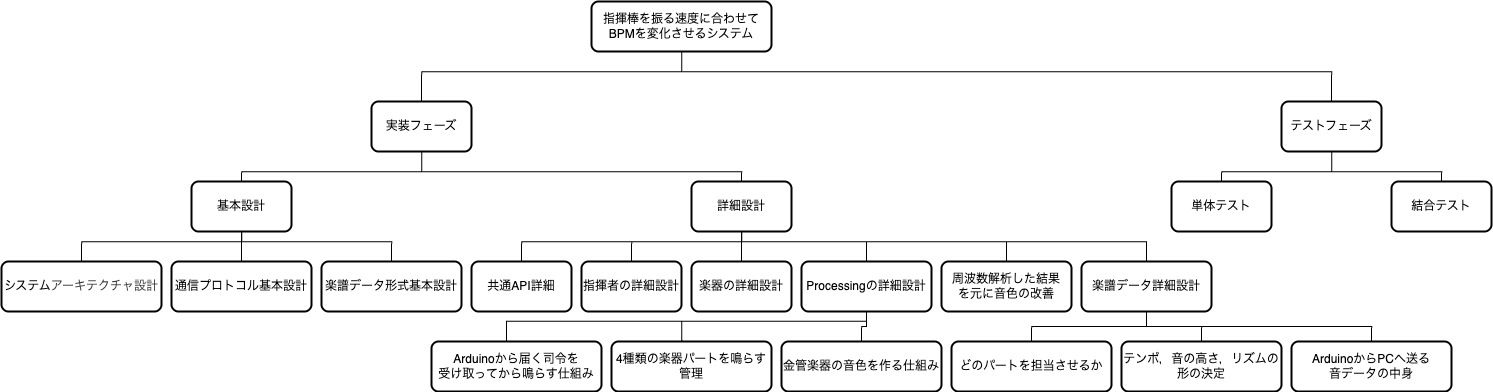
\includegraphics[width=15cm]{WBS.PNG}
\caption{本プロジェクトのWBS図}
\label{WBS}
\end{center}
\end{figure}

図\ref{WBS}は本プロジェクトのWBS図である．

最終的な役割分担，またそれぞれの工程でどれほど時間がかかるかの表は以下の表\ref{yakuwari}，表\ref{yakuwari_2}
に記載

\begin{table}[H]
\centering
\footnotesize % ここで文字を小さくする
\caption{新たに作成した作業分担表}
\renewcommand{\arraystretch}{0.9}
\label{yakuwari}
\begin{tabular}{|c|c|c|p{5cm}|c|c|}
\hline
時間的フェーズ & 番号 & 要素成果物 & 活動タスク & 担当者 & 必要時間 \\ \hline

% 設計フェーズ（合計14行）
\multirow{14}{*}{\shortstack{100 設計フェーズ \\ (3週間)}}
& 110 & 基本設計 & 111 FBSの最終化 & 全員 & 2日間 \\ \cline{4-6}
& & & 112 PBSの最終化 & 全員 & 2日間 \\ \cline{4-6}
& & & 112 MOE/MOP/TPMの最終化 & 全員 & 2日間 \\ \cline{4-6}
& & & 111 システムアーキテクチャ設計 & 塩澤 & 1週間 \\ \cline{4-6}
& & & 112 通信プロトコル基本設計 & 塩澤 & 1週間 \\ \cline{4-6}
& & & 113 楽譜データ形式基本設計 & 齊藤 & 2週間 \\ \cline{4-6}
& & & 114 音色合成基本設計 & 梅澤 & 2週間 \\ \cline{2-6}
& 120 & 詳細設計 & 121 共通層API詳細 & 塩澤 & 1週間 \\ \cline{4-6}
& & & 122 指揮者の詳細設計 & 塩澤 & 1週間 \\ \cline{4-6}
& & & 123 楽器の詳細設計 & 塩澤 & 1週間\\ \cline{4-6}
& & & 124 Arduinoから届く司令で鳴らす仕組み & 梅澤 & 2週間 \\ \cline{4-6}
& & & 125 4種類の楽器パートを鳴らす仕組み & 梅澤 & 2週間 \\ \cline{4-6}
& & & 126 楽器のような音色の作成 & 梅澤 & 2週間 \\ \cline{4-6}
& & & 127 楽器音を周波数分解し126にフィードバック & 齊藤 & 2週間 \\ \cline{4-6}
& & & 128 楽器パートの振り分け & 斎藤 & 3週間 \\ \cline{4-6}
& & & 129 テンポ，音の高さ，リズムの形の決定 & 斎藤 & 3週間 \\ \cline{4-6}
& & & 130 ArduinoからPCへ送る音データの中身 & 斎藤 & 3週間 \\ \hline

% 製造フェーズ（合計19行）
\multirow{19}{*}{\shortstack{200 製造フェーズ \\ (2週間)}}
& 210 & 共通層実装 & 211 IModule/ModuleTimer実装 & 塩澤 & 2週間 \\ \cline{4-6}
& & & 212 SystemData/ProjectConfig テンプレ整備 & 塩澤 & 2週間 \\ \cline{4-6}
& & & 213 OrcNetModule & 塩澤 & - \\ \cline{2-6}
& 220 & 指揮者 & 221 IMUドライバモジュール & 塩澤 & 2週間 \\ \cline{4-6}
& & & 222 信号前処理モジュール & 塩澤 & 2週間 \\ \cline{4-6}
& & & 223 拍検出モジュール & 塩澤 & 2週間 \\ \cline{4-6}
& & & 224 テンポ推定モジュール & 塩澤 & 2週間 \\ \cline{4-6}
& & & 225 コマンド送出モジュール & 塩澤 & 2週間 \\ \cline{2-6}
& 230 & 楽器 & 231 CTRL/BEAT受信モジュール & 塩澤 & 2週間 \\ \cline{4-6}
& & & 232 楽譜データ保持・進行ロジック & 塩澤 & 2週間 \\ \cline{4-6}
& & & 233 NOTE送出モジュール & 塩澤 & 2週間\\ \cline{4-6}
& & & 234 パート別差分適用 & 塩澤 & 2週間 \\ \cline{2-6}
& 240 & 楽譜準備 & 241 課題曲4パートの選定 & 齊藤 & 2週間 \\ \cline{4-6}
& & & 242 4パート楽譜のヘッダ配列化 & 齊藤 & 2週間 \\ \cline{4-6}
& & & 243 楽譜データのROM埋め込み確認 & 齊藤 & 2週間 \\ \cline{2-6}
& 250 & Processing実装 & 251 NOTE受信モジュール & 梅澤 & 2週間 \\ \cline{4-6}
& & & 252 金管音色合成エンジン & 梅澤 & 2週間 \\ \cline{4-6}
& & & 253 4パート同時発音管理 & 梅澤 & 2週間 \\ \cline{4-6}
& & & 254 UI/モード表示 & 梅澤 & 2週間 \\ \hline

\end{tabular}
\end{table}

\begin{table}[htbp]
\centering
\footnotesize % ここで文字を小さくする
\caption{新たに作成した作業分担表の続き}
\renewcommand{\arraystretch}{0.8}
\label{yakuwari_2}
\begin{tabular}{|c|c|c|p{5cm}|c|c|}
\hline
時間的フェーズ & 番号 & 要素成果物 & 活動タスク & 担当者 & 必要時間 \\ \hline

% テストフェーズ
\multirow{15}{*}{\shortstack{300 テストフェーズ \\ (2週間)}}
& 310 & 単体テスト & 311 共通層単体 & 塩澤 & 2週間 \\ \cline{4-6}
& & & 312 拍検出ゴールデンテスト & 塩澤 & 2週間 \\ \cline{4-6}
& & & 313 楽譜進行状態機械テスト & 塩澤 & 2週間 \\ \cline{4-6}
& & & 314 音色生成単体確認 & 梅澤 & 2週間 \\ \cline{2-6}
& 320 & 結合テスト & 321 指揮単体デモ & 塩澤 & 2週間 \\ \cline{4-6}
& & & 322 指揮者と楽器の結合 & 塩澤 & 2週間 \\ \cline{4-6}
& & & 323 ４ノード同期誤差計測 & 全員 & 2週間 \\ \cline{4-6}
& & & 324 全ノードとProcessing結合 & 全員 & 2週間 \\ \cline{2-6}
& 330 & システムテスト & 331 拍検出精度 & 塩澤 & 2週間 \\ \cline{4-6}
& & & 332 通信遅延 & 塩澤 & 2週間 \\ \cline{4-6}
& & & 333 動機誤差 & 全員 & 2週間 \\ \cline{4-6}
& & & 334 テンポ追従 & 塩澤 & 2週間 \\ \cline{4-6}
& & & 335 パケロス耐性 & 塩澤 & 2週間 \\ \cline{4-6}
& & & 336 CPU負荷 & 塩澤 &2週間 \\ \cline{4-6}
& & & 337 起動時間 & 塩澤 &2週間 \\ \hline

\multirow{3}{*}{400 ストレッチフェーズ}
& 410 & 強弱推定 & 411 velocity推定アルゴ実装 & 塩澤 & 1週間 \\ \cline{4-6}
& & & 412 CTRLパケットへのvelocity乗せこみ & 塩澤 & 1週間 \\ \cline{4-6}
& & & 413 強弱制御テスト & 塩澤 & 1週間 \\ \hline

\multirow{2}{*}{500 運用・発表}
& 510 & 発表 & 511 発表準備・デモ調整 & 全員 & 1週間 \\ \cline{2-6}
& 520 & 報告書 & 521 成果報告書(個人) & 全員 & 1週間 \\ \hline

\end{tabular}
\end{table}



%%%%%%%%%%%%%%%%%%%%%%%%
\subsection{アローダイアグラムとクリティカルパス}
以下にアローダイアグラムとクリティカルパスを添付する．
工程日数は工程の重さと担当者の技術を考慮し，バッファを持たせることで3ルートが同日で完了するよう調整した．
工程名の数字は表\ref{ganto}に記載される親タスクを参照している．
\begin{figure}[H]
\begin{center}

\includegraphics[width=16cm]{arrow.png}
\caption{アローダイアグラムとクリティカルパス}
\label{arrow}
\end{center}
\end{figure}

%%%%%%%%%%%%%%%%%%%%%%%%
\subsection{役割分担}
表\ref{yakuwari}，表\ref{yakuwari_2}のようになる．
%%%%%%%%%%%%%%%%%%%%%%%%
\subsection{ガントチャート}
\begin{figure}[H]
\begin{center}
\includegraphics[width=18cm]{ganto.png}
\caption{本プロジェクトのガントチャート}
\label{ganto}
\end{center}
\end{figure}
図\ref{ganto}は本プロジェクトのガントチャートである．
本プロジェクトでは，設計フェーズ，製造フェーズ，テストフェーズ，ストレッチフェーズ，運用・発表フェーズの順に作業を進める計画とした．

設計フェーズでは，FBS・PBS・MOE/MOP/TPMの最終化を行った後，システムアーキテクチャ設計や通信プロトコル設計，音色合成設計などの基本設計および詳細設計を実施する．

製造フェーズでは，共通層実装，指揮者ノード実装，楽器ノード実装，Processing側実装，楽譜データ準備を並行して進める．特に，拍検出モジュールやテンポ推定モジュール，音色合成エンジンなど，本システムの中核となる機能をこの期間に実装する．

テストフェーズでは，単体テスト，結合テスト，システムテストを段階的に実施する．単体テストでは各モジュール単位での動作確認を行い，結合テストでは指揮者ノード，楽器ノード，Processing間の連携動作を確認する．さらにシステムテストでは，拍検出精度，通信遅延，同期誤差，テンポ追従性能などを評価する．

ストレッチフェーズでは，余裕がある場合に強弱推定機能の追加実装を行う．最後に，運用・発表フェーズにおいてデモ調整および成果報告書作成を実施する計画である．

また，本ガントチャートでは複数の作業を並列に進行させることで，全13週間の期間内で効率的にシステム開発を進める構成としている．


%%%%%%%%%%%%%%%%%%%%%%%%
%%%%%%%%%%%%%%%%%%%%%%%%
\section{検証と妥当性確認: V\&V計画}
%%%%%%%%%%%%%%%%%%%%%%%%
\subsection{プロジェクトの成果物に対する有効指標MOE}
有効指標（MOE）は，システムが最終的にユーザー（指揮者・聴衆）に対して提供する価値を評価する指標である．
本プロジェクトでは，各テスト階層における性能指標（MOP)の達成を通じて，以下の3つの有効性を確立する．
\begin{table}[H]
  \centering
  \caption{MOEとMOPの対応関係および目標値}
  \begin{tabular}{|l|l|l|}
    \hline
    \textbf{有効指標 (MOE)} & \textbf{性能指標 (MOP)} & \textbf{目標値 / 達成水準} \\ \hline
    \multirow{3}{10em}{MOE 1: 音楽的再現性と正確性（単体テスト領域）} & 拍検出の正確性 & 正解率 $\ge 90\%$ \\ \cline{2-3}
    & 音階の誤差 & セント単位での許容範囲内 \\ \cline{2-3}
    & 楽譜との相違 & 誤ノート発音数 0 \\ \hline
    \multirow{3}{10em}{MOE 2: 合奏の一体感とインタラクティブ性（結合テスト領域）} & 楽器間同期誤差 & $\le 20$ ms \\ \cline{2-3}
    & 指揮から楽器への通信遅延 & $\le 30$ ms \\ \cline{2-3}
    & テンポ追従の遅延 & $\le 2$ 拍 \\ \hline
    \multirow{3}{10em}{MOE 3: システムとしての堅牢性と実用性（システムテスト領域）} & 起動時間 & $\le 5$ s \\ \cline{2-3}
    & CPU負荷 (入力フェーズ) & $\le 2$ ms \\ \cline{2-3}
    & パケットロスの許容範囲 & 演奏継続が可能なレベル \\ \hline
  \end{tabular}
\end{table}

%%%%%%%%%%%%%%%%%%%%%%%%
\subsection{有効指標MOEに対応する性能指標MOP}
前項で定義した各MOEに対し，システム全体として達成すべき性能指標を以下の通り定める．
これらは，特定の検証フェーズに限定されず，成果物が最終的に備えるべき技術的到達基準である．
\begin{itemize}
 \item{\textbf{音楽的品質の達成基準}}\\
  システムが「音楽」として機能するための基準である．指揮動作から拍を正確に解析し，指定された楽譜データを正確なピッチで物理的な音響・動作へと変換する精度を評価の主軸とする．
 \item{\textbf{リアルタイム・アンサンブルの達成基準}}\\
  システムが「合奏」および「指揮」として機能するための基準である．分散配置された複数ノード間での極小な同期誤差の維持，および指揮者の動的な変化（テンポ変化等）に対する停滞のない追従性能を評価の主軸とする．
 \item{\textbf{運用プラットフォームとしての達成基準}}\\
  システムが「実用的な道具」として機能するための基準である．限られた計算資源内での処理完結，無線環境下での通信断絶耐性，および即時稼働を可能にする運用性を評価の主軸とする．
\end{itemize}

%%%%%%%%%%%%%%%%%%%%%%%%
\subsection{システムテストで評価する性能指標MOP}
パケットロスの許容範囲は聴感破綻の発生が起きない5\%以内のパケットロスを指標とする．
CPUの負荷については，入力装置をしてから2ms以内を指標とする．

%%%%%%%%%%%%%%%%%%%%%%%%
\subsection{結合テストで評価する性能指標MOP}
通信の同期を行う際．20ms以内のズレであった場合は2つの音を別々に認識
できないため，同期の誤差を20ms以内を指標とする\cite{ref:douki}．

指揮棒から楽器への通信の遅延については，30ms以内を指標とする．

テンポの追従の遅延については，2拍以内を指標とする．
%%%%%%%%%%%%%%%%%%%%%%%%
\subsection{単体テストで評価する性能指標MOP}
拍検知の正確性については，90\%以上を指標とする．

音階の誤差については，自己相関による音階解析を行った際の，平均値が5.52centであった
ため，5.52centまでの誤差を指標とする\cite{ref:onkai}．
%%%%%%%%%%%%%%%%%%%%%%%%
\subsection{プロジェクト中に監視する技術性能指標TPM}
本項では，開発期間中において各性能指標の達成見込みを継続的に評価するための技術性能指標（TPM）を定義する．これらは，設計変更や機能実装に伴う技術的リスクを早期に発見することを目的として監視を行う．

\begin{itemize}
\item{\textbf{同期誤差の推移監視}}\\
最終目標値である 20 ms に対する現在の到達度を監視する．特に通信プロトコルの最適化やノード数の増減が発生した際に実測を行い，目標値からの乖離が10 ms以上となった場合には，バッファ制御アルゴリズムの再検討を実施する．
\item{\textbf{CPU処理時間のマージン監視}}\\
制御周期 5 ms に対する各タスクの処理時間を監視する．機能追加に伴いCPU負荷が目標値（2 ms）の 80 \% を超過した段階で，コードの最適化およびタスク優先順位の再設計を行い，リアルタイム性の破綻を未然に防止する．
\end{itemize}

%%%%%%%%%%%%%%%%%%%%%%%%
\subsection{プロジェクト中に監視する指標TPM}
技術的な数値指標に加え，プロジェクト全体の各システム性能を維持するために，リソースおよび進捗の観点から以下の指標を監視する．

\begin{itemize}
\item{\textbf{機能実装の完了率}}\\
WBSに基づく各モジュールの実装進捗を監視する．特に指揮解析と通信基盤の統合が予定より遅延した場合は，クリティカルパス上のリスクとして要員配置の再検討やスコープの調整を行う．
\item{\textbf{システム稼働の安定度}}\\
開発中の連続稼働テストにおける意図しないリセットやハングアップの発生頻度を監視する．ハードウェア起因の不安定要素やメモリリークを早期に特定・排除し，最終的なシステムテストにおける信頼性を担保する．
\end{itemize}



%%%%%%%%%%%%%%%%%%%%%%%%
%%%%%%%%%%%%%%%%%%%%%%%%
\section{資源・調達管理}
本節では，本プロジェクトの遂行に必要となるハードウェア資源および開発環境の調達計画について述べる．
\begin{itemize}
 \item{\textbf{ハードウェア資源}}\\
 本プロジェクトでは，計5台のArduino（指揮用1台，楽器用4台）を使用する．
 また，指揮解析用のIMUセンサおよび各楽器ノードの出力用デバイスについても，チーム内の既存資産および新規調達によって確保済みである．
 \item{\textbf{開発・運用リソース}}\\
 ソースコードの管理にはGitを用い，チーム内での並行開発を可能とする．
 また，無線通信環境の検証用として専用のルーターを用い，ハッカソン会場等の外部環境に依存しない安定した通信経路を確保する．
 
\end{itemize}


%%%%%%%%%%%%%%%%%%%%%%%%
%%%%%%%%%%%%%%%%%%%%%%%%
\section{リスク管理}
それぞれの担当箇所の作業日を長めに取ることで，病気や，不具合が発生し
作業が滞ったとしても，余分に作業日を設けているので
スケジュール通りの作業に修正することが容易になる．

%%%%%%%%%%%%%%%%%%%%%%%%
%%%%%%%%%%%%%%%%%%%%%%%%
%%%%%%%%%%%%%%%%%%%%%%%%
\chapter{システムの基本設計}



%%%%%%%%%%%%%%%%%%%%%%%%
\section{機能一覧}
\subsection{Processing音源サブシステム}
表\ref{tab:fbs}にProcessing音源サブシステムの機能一覧を示す．

\begin{longtable}{p{0.28\linewidth}p{0.62\linewidth}}
\caption{Processing 音源サブシステムの機能一覧}\label{tab:fbs}\\
\toprule
機能 & 役割 \\
\midrule
\endfirsthead
\toprule
機能 & 役割 \\
\midrule
\endhead
Serial 接続管理 &
Processing 起動時に Serial ポート一覧を表示し，画面上のポートをクリックして接続する．切断時は再接続待ちへ戻す． \\
NOTE フレーム同期・復号 &
USB Serial のバイト列から \texttt{magic=0x4F52} を探し，20 byte 固定長 NOTE に復号する． \\
パート設定管理 &
期待 \texttt{partId} を \texttt{0x02--0x05} から選び，誤接続時は発音せず警告とログを残す．検証用に ALL モードも持つ． \\
ボイス管理 &
NoteOn，NoteOff，\texttt{durationMs} 経過による自動消音，同時発音数上限，古い Voice の解放を管理する． \\
音色生成 &
\texttt{0x02--0x04} は金管音色，\texttt{0x05} はリズム音色として合成し，Minim の AudioOutput へ出力する． \\
UI 表示・操作 &
接続状態，期待 partId，受信数，破棄数，発音中 Voice 数，波形，警告を表示し，テスト発音やミュートを操作できるようにする． \\
ログ・検証支援 &
受信時刻，NOTE 内容，破棄理由，発音開始を CSV に記録し，結合試験で欠落や誤接続を確認できるようにする． \\
\bottomrule
\end{longtable}

\subsection{楽譜進行・発音情報配信}
以下に楽譜進行と発音情報配信に対応する表\ref{tab:functions}に機能一覧を示す．

\begin{longtable}{p{0.12\textwidth}p{0.22\textwidth}p{0.52\textwidth}}
\caption{担当範囲の機能一覧}\label{tab:functions}\\
\toprule
\textbf{ID} & \textbf{機能} & \textbf{役割} \\
\midrule
\endfirsthead
\toprule
\textbf{ID} & \textbf{機能} & \textbf{役割} \\
\midrule
\endhead
F3.2 & 楽譜データ保持 &
各楽器ノードが自分のパートの楽譜をC配列として保持する．外部ストレージは使用しない．\\
F3.3 & BEAT同期での音符進行 &
指揮者ノードから届くBEAT番号とマスタ時刻に合わせ，発火すべき楽譜イベントを選ぶ．\\
F3.4 & NOTEイベント生成 &
音符開始時にNoteOn，音符終了時にNoteOffを生成する．休符ではNOTEを送信しない．\\
F3.5 & パート固有ロジック &
\code{partId}，\code{startBeatNo}，楽譜配列をノードごとに差し替え，4声の輪唱とリズムを構成する．\\
F4.1 & NOTEパケット生成 &
発音情報を\code{partId}，\code{noteNumber}，\code{velocity}，\code{gate}，
\code{durationMs}へ変換する．\\
F4.2 & Processingへの送信 &
20バイト固定長のNOTEをUSB SerialでPCへ送信する．\\
\bottomrule
\end{longtable}



%%%%%%%%%%%%%%%%%%%%%%%%
\section{システム構成図}
\subsection{Processing音源サブシステム}
本番構成は，楽器ノード1台に対して Mac 1台を USB Serial で直結する構成である．
Processing は自分に接続された楽器ノードから NOTE を受け，音声出力を行う．

\begin{lstlisting}[style=textdiagram, caption={Processing 音源サブシステムを含む全体構成}, label={lst:overview}]
User conducts
    |
    v
node_01: conductor, CTRL/BEAT sender
    |
    | UDP multicast CTRL/BEAT
    v
node_02 -- USB Serial NOTE --> Mac 1 Processing final --> Brass 1
node_03 -- USB Serial NOTE --> Mac 2 Processing final --> Brass 2
node_04 -- USB Serial NOTE --> Mac 3 Processing final --> Brass 3
node_05 -- USB Serial NOTE --> Mac 4 Processing final --> Rhythm
\end{lstlisting}

\subsubsection{パート対応}
Processing は表\ref{tab:part-map}の対応で \texttt{partId} を解釈する．

\begin{longtable}{p{0.16\linewidth}p{0.14\linewidth}p{0.28\linewidth}p{0.32\linewidth}}
\caption{partId と音色・役割の対応}\label{tab:part-map}\\
\toprule
ノード & partId & 楽譜上の役割 & Processing 側音色 \\
\midrule
\endfirsthead
\toprule
ノード & partId & 楽譜上の役割 & Processing 側音色 \\
\midrule
\endhead
node\_02 & 0x02 & 主旋律 & Brass 1．基準となる金管音色． \\
node\_03 & 0x03 & 輪唱パート1 & Brass 2．金管音色を共有し，音量差で区別する． \\
node\_04 & 0x04 & 輪唱パート2 & Brass 3．金管音色を共有し，必要に応じて調整する． \\
node\_05 & 0x05 & ベース・リズム伴奏 & RhythmVoice．短い減衰を持つリズム音として鳴らす． \\
\bottomrule
\end{longtable}

\subsection{楽譜進行・発音情報配信}
ユーザは指揮者ノードを振る．指揮者ノードはBPMとBEATを楽器ノードへ送る．
楽器ノードは自分の楽譜を進め，PC上のProcessingへ発音情報を送る．
Processingは受け取ったNOTEから音を合成し，スピーカへ出力する．

\begin{figure}[H]
\centering
\resizebox{\linewidth}{!}{%
\begin{tikzpicture}[
  node distance=10mm and 14mm,
  box/.style={draw, rounded corners, align=center, minimum width=31mm, minimum height=10mm},
  small/.style={draw, rounded corners, align=center, minimum width=25mm, minimum height=9mm},
  arrow/.style={-{Latex[length=2.2mm]}, thick}
]
\node[box] (user) {ユーザ\\指揮を振る};
\node[box, right=of user] (conductor) {node\_01\\指揮者ノード};
\node[box, right=of conductor] (wifi) {WiFi UDP\\CTRL / BEAT};
\node[small, above right=4mm and 13mm of wifi] (n2) {node\_02\\金管1};
\node[small, right=13mm of wifi] (n3) {node\_03\\金管2};
\node[small, below right=4mm and 13mm of wifi] (n4) {node\_04\\金管3};
\node[small, below=13mm of n4] (n5) {node\_05\\ドラム};
\node[box, right=23mm of n3] (pc) {PC / Processing\\音色合成};
\node[box, right=of pc] (spk) {スピーカ\\演奏音};

\draw[arrow] (user) -- (conductor);
\draw[arrow] (conductor) -- (wifi);
\draw[arrow] (wifi) -- (n2);
\draw[arrow] (wifi) -- (n3);
\draw[arrow] (wifi) -- (n4);
\draw[arrow] (wifi) -- (n5);
\draw[arrow] (n2) -- node[above, font=\small]{NOTE} (pc);
\draw[arrow] (n3) -- (pc);
\draw[arrow] (n4) -- (pc);
\draw[arrow] (n5) -- (pc);
\draw[arrow] (pc) -- (spk);
\end{tikzpicture}
}
\caption{ユーザ目線のシステム構成}
\label{fig:system}
\end{figure}

\subsection{4パート振り分け}

課題曲候補は\textbf{「かえるのうた」}とする．輪唱しやすく，テンポ追従の確認がしやすいためである．
4パートの割り当てを表\ref{tab:part-assign}に示す．

\begin{table}[H]
\centering
\caption{4パート振り分け}
\label{tab:part-assign}
\begin{tabular}{p{0.13\textwidth}p{0.15\textwidth}p{0.13\textwidth}p{0.12\textwidth}p{0.35\textwidth}}
\toprule
\textbf{ノード} & \textbf{partId} & \textbf{役割} & \textbf{入り拍} & \textbf{楽譜内容} \\
\midrule
node\_02 & \code{0x02} & 金管1 & 0拍 & 主旋律を曲頭から演奏する．\\
node\_03 & \code{0x03} & 金管2 & 4拍 & 主旋律を4拍遅れて演奏する．\\
node\_04 & \code{0x04} & 金管3 & 8拍 & 主旋律を8拍遅れて演奏する．\\
node\_05 & \code{0x05} & ドラム & 0拍 & 1拍ごとのリズム伴奏を演奏する．\\
\bottomrule
\end{tabular}
\end{table}


%%%%%%%%%%%%%%%%%%%%%%%%
\section{操作インターフェース設計}
\subsection{Processing音源サブシステム}
Processing の利用者は，観客ではなく，デモ準備者または結合試験担当者である．
したがって UI は演奏表現ではなく，接続確認，異常検出，安全停止を目的とする．

\begin{longtable}{p{0.22\linewidth}p{0.26\linewidth}p{0.40\linewidth}}
\caption{Processing 側操作インターフェース}\label{tab:ui}\\
\toprule
操作・表示 & 対象 & システム挙動 \\
\midrule
\endfirsthead
\toprule
操作・表示 & 対象 & システム挙動 \\
\midrule
\endhead
起動 & Mac 担当者 & Serial ポート一覧を取得し，画面左に接続候補として表示する． \\
ポートクリック & Mac 担当者 & 選択した Serial ポートを開き，成功したら Ready へ遷移する． \\
\texttt{1}--\texttt{4} キー & Mac 担当者 & 期待 partId を 0x02--0x05 に切り替える．本番では Mac ごとに固定する． \\
\texttt{a} キー & 検証担当者 & ALL モードへ切り替え，0x02--0x05 の全パートを受け付ける． \\
\texttt{r} キー & Mac 担当者 & Serial を閉じ，ポート一覧を再列挙する． \\
\texttt{d} キー & Mac 担当者 & Serial を切断し，PortSelect へ戻す． \\
\texttt{m} キー & Mac 担当者 & ミュートを切り替える．ミュート時は既存 Voice を Release する． \\
\texttt{t} キー & Mac 担当者 & 選択中 partId のテスト音を鳴らし，スピーカと音量を確認する． \\
\texttt{g} キー & 検証担当者 & 疑似 NOTE フレームを内部注入し，Arduino なしで受信処理を確認する． \\
画面表示 & 全員 & 接続状態，期待 partId，受信数，破棄数，欠落数，Voice 数，波形，警告を表示する． \\
\bottomrule
\end{longtable}

\subsection{楽譜進行・発音情報配信}
\begin{table}[H]
\centering
\caption{ユーザ操作と楽器ノードの挙動}
\label{tab:user-flow}
\begin{tabular}{p{0.24\textwidth}p{0.31\textwidth}p{0.36\textwidth}}
\toprule
\textbf{ユーザ操作} & \textbf{入力される情報} & \textbf{楽器ノードの挙動} \\
\midrule
電源を入れる & USB給電，WiFi接続開始 & \code{Idle}から\code{WaitSync}へ進み，CTRL受信を待つ．\\
指揮を振り始める & BEATとBPMが届く & \code{startBeatNo}に達したパートから演奏を開始する．\\
速く振る／遅く振る & CTRLのBPM値が変化する & 次の音符から新しいBPMで発音長を計算する．\\
BEATが一時的に欠ける & BEAT未受信時間がしきい値を超える & 直前BPMで\code{SelfRun}し，実BEAT復帰後は通常演奏へ戻る．\\
曲が終わる & 最終イベントまで発火 & デモ時は曲頭へ戻り，ループ演奏する．\\
\bottomrule
\end{tabular}
\end{table}



%%%%%%%%%%%%%%%%%%%%%%%%
\section{状態遷移図}
\subsection{Processing音源サブシステム}
\begin{lstlisting}[style=textdiagram, caption={Processing 音源サブシステムの状態遷移}, label={lst:state}]
Boot
  -> PortSelect  : setup completed and serial ports listed
PortSelect
  -> Ready       : user clicks a serial port and open succeeds
  -> Error       : serial open fails
Ready
  -> Playing     : first valid NOTE received
  -> PortSelect  : user presses r or d
Playing
  -> Ready       : no NOTE for 1000 ms, serial still open
  -> PortSelect  : user presses r or d
  -> Error       : serial exception
Muted
  -> Playing     : user presses m again
  -> PortSelect  : user presses r or d
Error
  -> PortSelect  : user presses r
\end{lstlisting}

\begin{longtable}{p{0.18\linewidth}p{0.30\linewidth}p{0.40\linewidth}}
\caption{状態定義}\label{tab:states}\\
\toprule
状態 & 意味 & 主な処理 \\
\midrule
\endfirsthead
\toprule
状態 & 意味 & 主な処理 \\
\midrule
\endhead
Boot & 起動直後 & 画面，Minim，AudioOutput，Logger，PartManager，SerialFrameReader を初期化する． \\
PortSelect & Serial ポート選択待ち & ポート一覧を表示し，クリック入力を待つ． \\
Ready & 接続済み・NOTE 待ち & Serial バッファを空にし，NOTE の magic 同期を待つ． \\
Playing & 正常受信・発音中 & NOTE 復号，partId 検査，Voice 生成，ログ出力，画面更新を行う． \\
Muted & 受信継続・発音停止 & 新規 Voice は作らず，既存 Voice を Release する． \\
Error & 接続異常 & Serial を閉じ，未処理キューと受信バッファをクリアし，警告を表示する． \\
\bottomrule
\end{longtable}

\subsection{楽譜進行・発音情報配信}
\begin{figure}[H]
\centering
\resizebox{0.98\linewidth}{!}{%
\begin{tikzpicture}[
  state/.style={draw, rounded corners, align=center, minimum width=27mm, minimum height=10mm},
  edgeLabel/.style={font=\scriptsize, fill=white, inner sep=1.2pt},
  arrow/.style={-{Latex[length=2mm]}, thick}
]
\node[state] (idle) at (0,0) {Idle\\起動直後};
\node[state] (sync) at (4.3,0) {WaitSync\\時計同期待ち};
\node[state] (wait) at (8.6,0) {WaitStart\\入り拍待ち};
\node[state] (play) at (13.2,0) {Playing\\演奏中};
\node[state] (finish) at (8.6,-2.8) {Finished\\曲末};
\node[state] (self) at (13.2,-2.8) {SelfRun\\自走中};

\draw[arrow] (idle) -- node[above, edgeLabel]{WiFi接続} (sync);
\draw[arrow] (sync) -- node[above, edgeLabel]{CTRL受信} (wait);
\draw[arrow] (wait) -- node[above, edgeLabel]{開始拍に到達} (play);
\draw[arrow] (play) to[bend left=18] node[right, edgeLabel]{欠損} (self);
\draw[arrow] (self) to[bend left=18] node[left, edgeLabel]{復帰} (play);
\draw[arrow] (play.south west) -- ++(-1.1,-0.9) -- node[above, edgeLabel]{曲末} (finish.east);
\draw[arrow] (finish) -- node[left, edgeLabel]{ループ} (wait);
\end{tikzpicture}
}
\caption{楽器ノードの状態遷移}
\label{fig:state}
\end{figure}



%%%%%%%%%%%%%%%%%%%%%%%%
%%%%%%%%%%%%%%%%%%%%%%%%
%%%%%%%%%%%%%%%%%%%%%%%%

% === 塩澤担当：基本設計 ===

本章では，「Arduino オーケストラ」（指揮者ノード 1 + 楽器ノード 4 の計 5 ノード）のうち
塩澤担当範囲（指揮者ノード node\_01 と楽器ノード node\_02〜node\_05 のファームウェア）を
対象に，システム全体の機能・構成・操作インターフェース・状態遷移を基本設計レベルでまとめる．
楽器構成は \textbf{金管 3 + ドラム 1} とし，各楽器ノードは
\textbf{専用の Mac（Processing 実行）と 1 対 1 で USB 接続}される．Mac 側の
音色合成・スピーカ出力（梅澤担当），および楽譜を作る楽譜エディタ（齋藤担当）は本書のスコープ外で，
それぞれデータ受け渡し境界（NOTE パケット，楽譜データ形式）のみを定義する．通信は \textbf{ノード間（指揮者 → 楽器）= WiFi UDP マルチキャスト}，
\textbf{Arduino--Mac 間（楽器 → 各 Mac）= USB Serial（UART, \texttt{Serial.write}）}
の二系統に分離した構成を採る．

ファームウェアの設計原則は，外部 OSS であり著者本人が公開している
\textbf{Embedded-Module-Architecture（以下 EMA）}\footnote{\url{https://github.com/takushio2525/Embedded-Module-Architecture}}
に全面準拠する．EMA の中核ルール（\texttt{IModule} インターフェース，3 フェーズループ，
\texttt{SystemData} と \texttt{ProjectConfig} の集約）は \S\ref{sec:basic-architecture}
で位置づけを示し，第 \ref{chap:detail} 章で具体化する．


%%%%%%%%%%%%%%%%%%%%%%%%
\section{機能一覧}\label{sec:basic-functions}
%%%%%%%%%%%%%%%%%%%%%%%%

本節ではファームウェアが満たすべき要求と，それを機能分解構造（FBS）で整理した機能一覧を示す．
本書スコープは Arduino 系のファームウェアのみであり，楽器音色や発表準備などチーム全体側の要素は含めない．

\subsection{要求一覧}

本ファームウェアが満たすべき要求を表 \ref{tab:requirements} に示す．「(S)」はストレッチ要求
（必達機能の完成後に着手する）であり，R-Internal は外部から見えにくいが設計上必要な内部要求である．

\begin{longtable}{L{0.13\textwidth} L{0.27\textwidth} L{0.48\textwidth}}
\caption{要求一覧}\label{tab:requirements}\\
\toprule
\textbf{ID} & \textbf{要求} & \textbf{内容} \\
\midrule
\endfirsthead
\toprule
\textbf{ID} & \textbf{要求} & \textbf{内容} \\
\midrule
\endhead
R-1          & 5 台同期演奏   & 指揮者 1 + 楽器 4 の計 5 ノードが，指揮者の拍に合わせて同期して演奏する \\
R-2          & 輪唱曲の再生   & 主旋律 3 パート（金管）＋リズム 1 パート（ドラム）以上で構成される輪唱曲を演奏できる．各パートは入り拍をずらして輪唱になる \\
R-3          & 可変テンポ追従 & 指揮者の振りの速さの変化に楽器側のテンポが追従する \\
R-4 (S)      & 強弱制御       & 指揮者の振りの大きさに応じて発音の強弱（velocity）が変わる \\
R-Internal-1 & 通信の信頼性   & 数 \% 程度のパケロスが起きても演奏が破綻しない \\
R-Internal-2 & CPU リソース   & 各ノードが 200\,Hz の IMU サンプリングまたは UDP 受信を取りこぼさずに回せる範囲の処理量に収める \\
R-Internal-3 & 起動時間       & 電源投入から演奏可能になるまでが，実演のセットアップ時間として許容できる範囲（数秒）に収まる \\
\bottomrule
\end{longtable}

これらの要求に対する数値目標（設計目標値）は \S\ref{subsec:design-targets} に，検証の方向性は
\S\ref{sec:test-design} にまとめる．

\subsection{機能分解（FBS）}

\begin{description}
  \item[F1. 指揮情報抽出（node\_01）]
    F1.1 IMU 6 軸の取得，F1.2 信号前処理（IIR LPF + ノルム），
    F1.3 拍検出（振り下ろしピーク），F1.4 テンポ推定（拍間隔→BPM），
    F1.5 強弱推定（振幅→velocity，ストレッチ），F1.6 演奏状態管理．
  \item[F2. 指揮情報配信（node\_01）]
    F2.1 CTRL 送出（BPM・velocity・state），F2.2 BEAT 送出（拍トリガ），
    F2.3 SoftAP 起動・維持（自身がアクセスポイントを兼ね，楽器ノードを収容）．
  \item[F3. 楽譜進行（node\_02〜05）]
    F3.1 CTRL/BEAT 受信，F3.2 楽譜データ保持（C 配列・パート別），
    F3.3 BEAT 同期での音符進行，F3.4 NOTE イベント生成，
    F3.5 パート固有ロジック（\texttt{PART\_ID}・\texttt{startBeatNo}）．
  \item[F4. 発音情報配信（node\_02〜05 → PC）]
    F4.1 NOTE パケット生成，F4.2 Processing への USB Serial 送信
    （\texttt{Serial.write()}，CDC 1:1 接続）．
  \item[F5. 共通基盤（全ノード）]
    F5.1 \texttt{IModule} 登録・3 フェーズループ，
    F5.2 \texttt{ModuleTimer} による周期実行，
    F5.3 \texttt{SystemData}/\texttt{ProjectConfig} 集約，
    F5.4 起動シーケンス・診断 LED，
    F5.5 init 失敗リトライ・パケロス時のフォールバック．
\end{description}

ストレッチ機能（F1.5 強弱推定）は必達機能の実装完了後に着手する．
詳細設計ではインターフェースだけ用意し，初期実装ではスタブで通す構成にする．


%%%%%%%%%%%%%%%%%%%%%%%%
\section{システム構成図}\label{sec:basic-architecture}
%%%%%%%%%%%%%%%%%%%%%%%%

\subsection{全体ブロック図}

5 ノードと Mac × 4 の関係を図 \ref{fig:overview} に示す．\textbf{指揮者 node\_01 自身が
SoftAP（ESP32-S3 のソフトウェア AP）を立て}，楽器 node\_02〜05 は STA としてこれに
接続する．外部ルータやスマホテザリングは不要．node\_01 は CTRL/BEAT を
\textbf{UDP マルチキャスト} で送信し，node\_02〜05 はそれぞれグループに join して受信する．
各楽器は楽譜を進行させながら NOTE を \textbf{USB Serial}（\texttt{Serial.write}）で
\textbf{専用 Mac（1 対 1 接続）} へ送信する．Arduino--Mac 間は WiFi を介さず，給電と
Serial 通信を兼ねた USB 接続で直結する．

\begin{figure}[H]
\centering
\begin{tikzpicture}[
  node distance=8mm and 30mm,
  node_box/.style={draw=black, fill=codebg, rounded corners=2pt, minimum width=22mm, minimum height=9mm, align=center, font=\small},
  ap_box/.style  ={draw=black, thick, fill=lightgray, rounded corners=2pt, minimum width=30mm, minimum height=14mm, align=center, font=\small},
  pc_box/.style  ={draw=black, fill=lightgray, rounded corners=2pt, minimum width=18mm, minimum height=9mm, align=center, font=\small},
  arr/.style     ={-{Stealth[length=2mm]}, thick, black},
  arr2/.style    ={-{Stealth[length=2mm]}, thick, black, dashed},
  lbl/.style     ={font=\scriptsize, align=center, fill=white, inner sep=1pt},
]
  \node[node_box]              (n2)                                  {node\_02\\金管 1};
  \node[node_box, below=of n2] (n3)                                  {node\_03\\金管 2};
  \node[node_box, below=of n3] (n4)                                  {node\_04\\金管 3};
  \node[node_box, below=of n4] (n5)                                  {node\_05\\ドラム};
  \node[ap_box]                (n1) at ($(n3)!0.5!(n4) + (-50mm,0)$) {node\_01\\XIAO ESP32-S3 Sense\\+ MPU6050\\\textbf{（SoftAP）}};
  \node[pc_box, right=of n2]   (pc1)                                 {Mac 1};
  \node[pc_box, right=of n3]   (pc2)                                 {Mac 2};
  \node[pc_box, right=of n4]   (pc3)                                 {Mac 3};
  \node[pc_box, right=of n5]   (pc4)                                 {Mac 4};

  \draw[arr] (n1) -- node[lbl, pos=0.55] {CTRL/BEAT\\(UDP Mcast)} (n2);
  \draw[arr] (n1) -- (n3);
  \draw[arr] (n1) -- (n4);
  \draw[arr] (n1) -- (n5);
  \draw[arr2] (n2) -- node[lbl, pos=0.5] {NOTE\\(UART)} (pc1);
  \draw[arr2] (n3) -- (pc2);
  \draw[arr2] (n4) -- (pc3);
  \draw[arr2] (n5) -- (pc4);
\end{tikzpicture}
\caption{全体ブロック図（指揮者 node\_01 が SoftAP を兼ね，楽器 4 台が STA 接続．実線＝WiFi UDP マルチキャスト，破線＝楽器 → Mac の 1 対 1 USB Serial）}\label{fig:overview}
\end{figure}

\subsection{ノード役割分担}

各ノードの責務とコード担当者を表 \ref{tab:node-roles} に示す．node\_02〜05 の Arduino
コードは \textbf{共通ソース + パート設定差し替え}（\texttt{ProjectConfig} と楽譜データのみ差分）
で構成し，4 台分の別コードは書き分けない（\S\ref{sec:proc-flow-performer}）．

\begin{longtable}{l p{0.20\textwidth} p{0.42\textwidth} l}
\caption{ノード役割分担}\label{tab:node-roles}\\
\toprule
\textbf{ノード} & \textbf{物理配置} & \textbf{主な責務} & \textbf{コード担当} \\
\midrule
\endfirsthead
\toprule
\textbf{ノード} & \textbf{物理配置} & \textbf{主な責務} & \textbf{コード担当} \\
\midrule
\endhead
node\_01 & 指揮者の手・指揮棒 & MPU6050 読み取り → 拍・テンポ・強弱推定 → CTRL/BEAT 送出．\textbf{自身が SoftAP を起動}し楽器を収容 & 塩澤 \\
node\_02 & 金管 1             & BEAT 同期で楽譜進行 → NOTE 送出（金管 1 パート） & 塩澤 \\
node\_03 & 金管 2             & BEAT 同期で楽譜進行 → NOTE 送出（金管 2 パート） & 塩澤 \\
node\_04 & 金管 3             & BEAT 同期で楽譜進行 → NOTE 送出（金管 3 パート） & 塩澤 \\
node\_05 & ドラム             & BEAT 同期で楽譜進行 → NOTE 送出（ドラム） & 塩澤 \\
Mac $\times$ 4 & 楽器ごとに 1 台 & UART で NOTE を受信 → 倍音・ADSR 調整 → 波形生成 → 内蔵スピーカ出力 & 梅澤（参考） \\
\bottomrule
\end{longtable}

\subsection{データフロー}

演奏中の 1 拍ぶんの情報の流れを擬似シーケンスで示す．

\begin{notebox}
\textbf{1 拍ぶんのデータフロー（演奏中）}\\[2pt]
(1) MPU6050（I2C）$\to$ node\_01: 加速度・角速度サンプル（200 Hz）．\\
(2) node\_01 内: \texttt{applyPattern()} がフィルタ・拍検出・テンポ推定を実行．\\
(3) 振り下ろしを検出: node\_01（SoftAP）$\to$ node\_02〜05 に \textbf{BEAT}
   （\texttt{beatNo}, \texttt{timestampMs}）を UDP マルチキャスト．\\
(4) node\_02〜05 内: 受信 BEAT の \texttt{beatNo} から楽譜位置を算出 $\to$ NoteOn フラグ設定．\\
(5) node\_02〜05 $\to$ \textbf{各 Mac（1 対 1）}: \textbf{NOTE}
   （\texttt{noteNumber}, \texttt{velocity}, \texttt{durationMs}）を
   USB Serial（\texttt{Serial.write}）で送信．\\
(6) 並行して node\_01 は 20 Hz で \textbf{CTRL}（BPM・velocity・state）を
   同じマルチキャストグループへ送信し続ける．
\end{notebox}

\subsection{採用アーキテクチャ（EMA）の方針}

全 5 ノードのファームウェアは EMA に準拠する．EMA の中核ルールを本ハッカソンに
当てはめた要旨を以下に示す．バイト単位のパケット定義や具体コードは
第 \ref{chap:detail} 章で示す．

\begin{itemize}
  \item \textbf{\texttt{IModule} インターフェース}: 全ハードウェアモジュールが
        \texttt{init()} / \texttt{updateInput()} / \texttt{updateOutput()} / \texttt{deinit()}
        の 4 メソッドを実装する．
  \item \textbf{3 フェーズ実行モデル}: \texttt{loop()} は
        「入力 $\to$ ロジック \texttt{applyPattern()} $\to$ 出力」の順で必ず実行する．
  \item \textbf{\texttt{SystemData} 集約}: モジュール間共有状態を一元化する構造体．
        モジュール同士の直接呼び出しは禁止．
  \item \textbf{\texttt{ProjectConfig} 集約}: 各モジュールの設定を
        \texttt{\{MODULE\}\_CONFIG} インスタンスとして 1 ヘッダに集約．
  \item \textbf{判断ロジックの位置づけ}: 拍検出・テンポ推定・楽譜進行のような
        「ハードウェアに触れない判断ロジック」は \texttt{IModule} の派生にせず，
        \texttt{applyPattern()} 関数内に書く．
\end{itemize}


%%%%%%%%%%%%%%%%%%%%%%%%
\section{操作インターフェース設計}\label{sec:basic-ui}
%%%%%%%%%%%%%%%%%%%%%%%%

本節では「操作インターフェース」を，\textbf{ユーザーが触れる物理 IF}（指揮棒・LED）と
\textbf{ノード間／PC 間の通信プロトコル IF}（CTRL/BEAT/NOTE）の二層に分けて定義する．
通信は \textbf{Arduino--Arduino 間 = WiFi UDP}，\textbf{Arduino--PC 間 = USB Serial}
の二系統に分け，それぞれ役割と性質が異なる．バイト単位のパケットレイアウトは
\S\ref{sec:func-design} で具体化する．

\subsection{ユーザー操作}

\begin{itemize}
  \item \textbf{指揮棒（指揮者）}: MPU6050 を搭載した node\_01（XIAO ESP32-S3 Sense）を指揮棒として手に持ち，
        通常の指揮動作（4 拍子・3 拍子の振り下ろし）で操作する．特別なボタン等は持たない．
  \item \textbf{起動順}: 楽器ノード（node\_02〜05）を先に起動し（\texttt{Idle} 状態で
        SoftAP を待機），その後に指揮者ノード（node\_01）を起動する．指揮者の SoftAP
        起動で楽器が \texttt{WaitStart} に遷移し，指揮者の \texttt{Conducting} 入りで
        BEAT が流れ始めて楽器が \texttt{Playing} に遷移する．
  \item \textbf{Calibrating}: 指揮者ノードは起動後，最初の 2 秒間に静止時の加速度ノルム
        （$\approx$ 重力 1\,g）を平均して記録する．使用者は単に「起動後 2 秒間，腕を自然に下ろした状態で
        待つ」だけでよい．
\end{itemize}

\subsection{LED 表示仕様}

各ノードは内蔵 LED（\texttt{LED\_BUILTIN}）の点滅パターンで状態を提示する
（表 \ref{tab:led-spec}）．点滅周期は \texttt{StatusLedConfig.blinkIntervalMs} で調整可能．

\begin{longtable}{p{0.15\textwidth} p{0.18\textwidth} p{0.20\textwidth} p{0.36\textwidth}}
\caption{LED 表示パターン}\label{tab:led-spec}\\
\toprule
\textbf{ノード} & \textbf{状態} & \textbf{LED パターン} & \textbf{意味} \\
\midrule
\endfirsthead
\toprule
\textbf{ノード} & \textbf{状態} & \textbf{LED パターン} & \textbf{意味} \\
\midrule
\endhead
node\_01     & Idle        & 低速点滅（1 Hz）   & 起動直後・SoftAP 起動前 \\
node\_01     & Calibrating & 中速点滅（2 Hz）   & 停止時ノルムの学習中（2 秒） \\
node\_01     & Conducting  & 点灯               & 通常演奏中 \\
node\_01     & Fallback    & 高速点滅（5 Hz）   & IMU エラー or SoftAP 異常 \\
node\_02--05 & Idle        & 低速点滅（1 Hz）   & 起動直後・SoftAP 未接続 \\
node\_02--05 & WaitStart   & 中速点滅（2 Hz）   & SoftAP 接続済，最初の BEAT 待ち \\
node\_02--05 & Playing     & 点灯               & 通常演奏中（次 BEAT が長く来なくても Playing に留まる） \\
\bottomrule
\end{longtable}

\subsection{通信プロトコル方針（CTRL / BEAT / NOTE）}\label{subsec:protocol-policy}

3 種類のメッセージを使い分ける（表 \ref{tab:msg-policy}）．

\begin{longtable}{l p{0.27\textwidth} p{0.16\textwidth} p{0.13\textwidth} p{0.22\textwidth}}
\caption{3 種類のメッセージの設計方針}\label{tab:msg-policy}\\
\toprule
\textbf{種別} & \textbf{送信元 → 宛先} & \textbf{送信契機} & \textbf{性質} & \textbf{役割} \\
\midrule
\endfirsthead
\toprule
\textbf{種別} & \textbf{送信元 → 宛先} & \textbf{送信契機} & \textbf{性質} & \textbf{役割} \\
\midrule
\endhead
CTRL & node\_01 → node\_02--05 (UDP Mcast)        & 定期（20 Hz）       & 冪等         & BPM・velocity・state を継続同期 \\
BEAT & node\_01 → node\_02--05 (UDP Mcast)        & 拍検出時（不定期） & 即時性重視   & 楽譜ポインタ前進トリガ \\
NOTE & node\_02--05 → 各 Mac (USB Serial, 1:1)    & 楽譜イベント発火時 & 順序保証     & 自パート Mac への発音依頼 \\
\bottomrule
\end{longtable}

\textbf{設計原則}:
\begin{itemize}
  \item \textbf{CTRL は冪等}: 取りこぼしてもすぐ次が来るため，パケロス耐性は通信方針側で確保される．
  \item \textbf{BEAT は即時}: 1 拍 1 発が原則．確実性を上げるため同一 \texttt{beatNo} を
        \texttt{beatRedundancy} 回（既定 2）連送し，受信側で \texttt{beatNo} 重複排除する（冪等処理）．
  \item \textbf{BEAT が来ない間も留まる}: 楽器は仮想 BEAT を内挿して走り続けず，BEAT が長く来なくても
        \texttt{Playing} に留まって次の BEAT 到来時に自然再開する．連送（\texttt{beatRedundancy}）と
        過去 BEAT の即発火で取りこぼしを吸収する．
  \item \textbf{NOTE は単一経路}: 楽器 → 自パート Mac で 1 系統．楽譜に従って必ず送出する．
        Arduino--Mac 間は 1 対 1 USB Serial 直結のため，パケロスやネットワーク輻輳の心配なく
        確定到達するのが利点．
\end{itemize}

\subsection{通信方式（WiFi UDP + USB Serial の二系統）}

通信仕様を表 \ref{tab:net-spec} に示す．運用時に変わる値（SSID／パス）は
\texttt{OrcNetConfig} のリテラルで一元管理する．

\begin{longtable}{p{0.26\textwidth} p{0.66\textwidth}}
\caption{通信仕様}\label{tab:net-spec}\\
\toprule
\textbf{項目} & \textbf{設計} \\
\midrule
\endfirsthead
\toprule
\textbf{項目} & \textbf{設計} \\
\midrule
\endhead
ノード間（CTRL/BEAT）    & WiFi UDP．node\_01 → node\_02--05 へ \textbf{UDP/5001 マルチキャスト}（仮 \texttt{239.0.0.1}）．楽器側は \texttt{WiFiUDP.beginMulticast()} でグループに join \\
WiFi モード              & \textbf{node\_01 が SoftAP（\texttt{WiFi.softAP()}）}，node\_02--05 が STA（\texttt{WiFi.begin()}）として接続．外部ルータ・テザリング不要 \\
SSID / パス             & 仮 \texttt{OrchestraAP} / \texttt{orchestra2026}（node\_01 が公開し，node\_02--05 が同設定で接続）．本番運用で差替え \\
IP 割り当て              & node\_01 は SoftAP の既定 \texttt{192.168.4.1}．node\_02--05 は SoftAP 内蔵 DHCP で \texttt{192.168.4.2--5} を自動取得 \\
Arduino--Mac 間（NOTE）  & \textbf{USB Serial（CDC, \texttt{Serial.write}）}．\textbf{各楽器ノードと専用 Mac が 1 対 1} で USB 接続．Mac 側 Processing は対応する 1 ポートだけを開く \\
ボーレート               & 115200 bps．USB CDC ではボーレート設定は実質無視される（\texttt{NoteSenderConfig.baudRate} に形式上の値として 115200 を入れておくだけで，通信速度には影響しない） \\
フレーミング             & 全パケットの先頭 12 B 共通ヘッダの \texttt{magic = 0x4F52} がフレーム同期マークを兼ねる（\S\ref{sec:func-design}） \\
エンディアン             & リトルエンディアン（ESP32-S3 Xtensa LX7 / RA4M1 Cortex-M4 とも同一） \\
\bottomrule
\end{longtable}

\subsection{パケロス・ジッタ対策}

\begin{itemize}
  \item \textbf{CTRL 取りこぼし}: 冪等かつ 20 Hz 定期送信なので設計上問題にならない．
  \item \textbf{BEAT 取りこぼし}: 同一 BEAT を \texttt{beatRedundancy} 回（既定 2）連送し，楽器側で
        \texttt{beatNo} の重複を排除する．楽譜進行は \texttt{beatNo} 駆動（\S\ref{sec:proc-flow-performer}）のため，
        連送が両方落ちて 1 拍ぶん欠落しても，その次の BEAT の \texttt{beatNo} から算出される楽譜位置は
        欠落ぶんだけ正しく進んでおり自己修復する．BEAT が長く来なくても楽器は \texttt{Playing} に留まり，
        次の BEAT 到来時に自然再開する（仮想 BEAT を内挿して走り続ける方式は，指揮者の再起動中などに
        楽器だけが暴走する危険があるため採らない）．
  \item \textbf{ジッタ（楽器間同期誤差）}: BEAT 受信時刻ではなく
        \textbf{マスタ時刻 \texttt{playAtMasterMs} で発音タイミングを揃える}
        （\S\ref{subsec:clock-sync}）．WiFi の到達時刻ばらつきは時計オフセット推定の
        誤差に押し付けられ，同期収束後の定常状態では 4 台の発音差は設計目標の 20\,ms 以内に収まる見込み．
        ただし「鳴らない」を最優先して過去時刻の BEAT も即発火するため，ある 1 台だけ受信が大きく遅れた拍は
        その台の発音だけが一時的にずれる（詳細と条件の切り分けは \S\ref{subsec:clock-sync}）．
  \item \textbf{プロトコル不整合}: \texttt{magic} / \texttt{version} 不一致のパケットは破棄し，
        \texttt{StatusLedModule} が \texttt{data.orcNet} を読んで点滅パターンに反映する．
\end{itemize}


%%%%%%%%%%%%%%%%%%%%%%%%
\section{状態遷移図}\label{sec:basic-state}
%%%%%%%%%%%%%%%%%%%%%%%%

各ノード種ごとの演奏状態を 4 状態の有限状態機械として定義する．状態は
\texttt{ConductorState}（指揮者）と \texttt{PerformerState}（楽器）の
\texttt{enum class} として \texttt{SystemData} の中に保持し，
\texttt{applyPattern()} が遷移を判定する．

\subsection{指揮者ノード（node\_01）}

\begin{figure}[H]
\centering
\begin{tikzpicture}[
  node distance=14mm and 28mm,
  state/.style={draw=black, fill=codebg, rounded corners=2pt, minimum width=24mm, minimum height=10mm, align=center, font=\small},
  arr/.style ={-{Stealth[length=2.5mm]}, thick, black, font=\scriptsize},
  lbl/.style ={font=\scriptsize, fill=white, inner sep=1pt, align=center},
]
  \node[state] (idle)                       {Idle};
  \node[state, right=of idle] (cal)         {Calibrating};
  \node[state, right=of cal]  (cond)        {Conducting};
  \node[state, below=of cond] (fb)          {Fallback};

  \draw[arr] (idle)  --                node[lbl]                {SoftAP\\起動完了}    (cal);
  \draw[arr] (cal)   --                node[lbl]                {2 秒経過}            (cond);
  \draw[arr] (cond)  --                node[lbl, right=1pt]     {IMU/WiFi エラー}     (fb);
  \draw[arr] (fb)    to[bend left=30]  node[lbl, left=1pt]      {復旧}                 (cond);
\end{tikzpicture}
\caption{指揮者ノードの状態遷移}\label{fig:state-conductor}
\end{figure}

\begin{longtable}{p{0.13\textwidth} p{0.34\textwidth} p{0.44\textwidth}}
\caption{指揮者ノードの状態定義}\label{tab:state-conductor}\\
\toprule
\textbf{状態} & \textbf{意味} & \textbf{動作} \\
\midrule
\endfirsthead
\toprule
\textbf{状態} & \textbf{意味} & \textbf{動作} \\
\midrule
\endhead
Idle        & 起動直後．SoftAP 起動前     & ImuModule.updateInput は動くが拍検出は無効．OrcSenderModule は何も送らない \\
Calibrating & 初期静止状態の学習中（2 秒） & applyPattern() が生加速度ノルムの平均を停止時ノルムとして記録 \\
Conducting  & 通常演奏中                 & 全モジュール稼働．BEAT を拍検出時に送出，CTRL を 20 Hz 周期で送出 \\
Fallback    & エラー発生                 & CTRL は state=Fallback で送り続ける．BEAT は停止．LED 高速点滅 \\
\bottomrule
\end{longtable}

\subsection{楽器ノード（node\_02〜05）}

\begin{figure}[H]
\centering
\begin{tikzpicture}[
  node distance=14mm and 32mm,
  state/.style={draw=black, fill=codebg, rounded corners=2pt, minimum width=24mm, minimum height=10mm, align=center, font=\small},
  arr/.style ={-{Stealth[length=2.5mm]}, thick, black, font=\scriptsize},
  lbl/.style ={font=\scriptsize, fill=white, inner sep=1pt, align=center},
]
  \node[state] (idle)                       {Idle};
  \node[state, right=of idle] (wait)        {WaitStart};
  \node[state, right=of wait] (play)        {Playing};

  \draw[arr] (idle)  --                node[lbl]              {WiFi 接続完了}             (wait);
  \draw[arr] (wait)  --                node[lbl]              {最初の BEAT 受信}         (play);
\end{tikzpicture}
\caption{楽器ノードの状態遷移（3 状態構成）}\label{fig:state-performer}
\end{figure}

\begin{longtable}{p{0.13\textwidth} p{0.34\textwidth} p{0.44\textwidth}}
\caption{楽器ノードの状態定義}\label{tab:state-performer}\\
\toprule
\textbf{状態} & \textbf{意味} & \textbf{動作} \\
\midrule
\endfirsthead
\toprule
\textbf{状態} & \textbf{意味} & \textbf{動作} \\
\midrule
\endhead
Idle      & 起動直後．node\_01 SoftAP 未接続 & 受信モジュールは動くが楽譜進行ロジックは無効．SoftAP に接続できるまでリトライ \\
WaitStart & SoftAP 接続済，最初の BEAT 待ち & CTRL/BEAT を受信し時計オフセットの EMA 学習を開始する．\textbf{時計同期の収束は Playing 遷移条件にしない}（収束待ちで遷移をブロックすると音が出なくなりやすいため）．最初の数拍は受信遅延ぶんのズレが残るが，CTRL を数発受けたあとに \texttt{offsetMs} が自然収束する \\
Playing   & 通常演奏中                 & BEAT 受信ごとに，その \texttt{beatNo} から楽譜位置（\texttt{(beatNo - startBeatNo) mod kScoreLength}）を算出して NOTE を送出．BEAT が長く来なくても \texttt{Playing} に留まり，次の BEAT で自然再開する \\
\bottomrule
\end{longtable}


%%%%%%%%%%%%%%%%%%%%%%%%
%%%%%%%%%%%%%%%%%%%%%%%%
%%%%%%%%%%%%%%%%%%%%%%%%
\chapter{システムの詳細設計}


%%%%%%%%%%%%%%%%%%%%%%%%
\section{部品一覧}
製品分解構造PBSの要素の説明

%%%%%%%%%%%%%%%%%%%%%%%%
%%%%%%%%%%%%%%%%%%%%%%%%
\section{ハードウェア設計}
\subsection{Processing音源サブシステム}
Processing 側では回路を追加しないが，接続される構成要素と故障時動作を明確化する．

\begin{longtable}{p{0.28\linewidth}p{0.12\linewidth}p{0.50\linewidth}}
\caption{Processing 側関連部品}\label{tab:parts}\\
\toprule
要素 & 数量 & 役割 \\
\midrule
\endfirsthead
\toprule
要素 & 数量 & 役割 \\
\midrule
\endhead
Arduino UNO R4 WiFi & 4 & node\_02--05．楽譜進行後，NOTE パケットを USB Serial で送信する． \\
Mac & 4 & Processing 実行機．本番は1台につき1つの Serial ポートを開く． \\
USB Type-C ケーブル & 4 & Arduino と Mac の給電および Serial 通信を兼ねる． \\
スピーカまたは内蔵スピーカ & 4 & Processing の AudioOutput を再生する． \\
Processing 4 + Minim & 4環境 & NOTE を受けて音を合成する実行環境． \\
\bottomrule
\end{longtable}

\begin{longtable}{p{0.24\linewidth}p{0.64\linewidth}}
\caption{Processing 側ハードウェア接続設計}\label{tab:hw-design}\\
\toprule
項目 & 設計 \\
\midrule
\endfirsthead
\toprule
項目 & 設計 \\
\midrule
\endhead
接続方式 & node\_02--05 と Mac 1--4 を USB Type-C で 1 対 1 接続する． \\
通信方式 & USB CDC Serial．Arduino 側は \texttt{Serial.write()} で NOTE を20 byte固定長バイナリとして送る． \\
ボーレート & 115200 bps．Arduino 側の NoteSender 設定と統一する． \\
フレーミング & 全 NOTE は先頭2 byte の \texttt{magic=0x4F52} を同期マークとする．Serial 上では \texttt{0x52 0x4F} の順に現れる． \\
音声出力 & 各 Mac の既定オーディオ出力へ送る．本番前に OS 音量と Processing 側ゲインを確認する． \\
誤接続対策 & Mac ごとに期待 \texttt{partId} を設定し，異なる \texttt{partId} は発音せず警告とログを残す． \\
切断時動作 & Serial 切断または例外時はポートを閉じ，受信キューとバッファをクリアし，全 Voice を停止する． \\
\bottomrule
\end{longtable}
%%%%%%%%%%%%%%%%%%%%%%%%%%%%%%%%%%%%%%%%%%%%%%%%%%%%%%%%%
\subsection{楽譜進行・発音情報配信}
本範囲で直接追加する部品はないが，楽譜データとNOTE送信が前提とする機器，
接続関係，動作条件を表\ref{tab:hardware}と図\ref{fig:hardware}に示す．

\begin{longtable}{p{0.20\textwidth}p{0.23\textwidth}p{0.47\textwidth}}
\caption{使用する機器と役割}\label{tab:hardware}\\
\toprule
\textbf{機器} & \textbf{型番・構成} & \textbf{役割} \\
\midrule
\endfirsthead
\toprule
\textbf{機器} & \textbf{型番・構成} & \textbf{役割} \\
\midrule
\endhead
楽器ノード & Arduino UNO R4 WiFi × 4 & \code{node\_02}〜\code{node\_05}．楽譜配列を保持し，NOTEを送信する．\\
指揮者ノード & Arduino系マイコン × 1 & CTRL / BEATをWiFi UDPで配信する．楽譜データは保持しない．\\
PC & MacまたはPC × 1〜4 & Processingを実行し，USB SerialからNOTEを受け取る．\\
接続ケーブル & USB Type-C等 & 楽器ノードとPCを1対1，またはUSBハブ経由で接続する．\\
音声出力 & PC内蔵または外部スピーカ & Processingが合成した音を出力する．\\
ストレージ & 追加なし & 楽譜はArduinoのプログラムメモリに埋め込むため，SDカードは使わない．\\
\bottomrule
\end{longtable}

\begin{figure}[H]
\centering
\resizebox{0.95\linewidth}{!}{%
\begin{tikzpicture}[
  node distance=10mm and 16mm,
  box/.style={draw, align=center, minimum width=34mm, minimum height=10mm},
  arrow/.style={-{Latex[length=2.2mm]}, thick}
]
\node[box] (n1) {node\_01\\CTRL / BEAT送信};
\node[box, right=of n1] (n) {node\_02〜05\\楽譜配列 + NOTE生成};
\node[box, right=of n] (pc) {PC\\Processing};
\node[box, right=of pc] (spk) {スピーカ};
\draw[arrow] (n1) -- node[above, font=\small]{WiFi UDP} (n);
\draw[arrow] (n) -- node[above, font=\small]{USB Serial 20B NOTE} (pc);
\draw[arrow] (pc) -- node[above, font=\small]{音声信号} (spk);
\end{tikzpicture}
}
\caption{ハードウェア接続関係}
\label{fig:hardware}
\end{figure}
%%%%%%%%%%%%%%%%%%%%%%%%%%%%%%%%%%%%%%%%%%%%%%%%%%%%%%%%%

%%%%%%%%%%%%%%%%%%%%%%%%
%%%%%%%%%%%%%%%%%%%%%%%%
\section{ソフトウェア設計}
\subsection{Processing音源サブシステム}
\subsubsection{NOTE パケット設計}
Processing は表\ref{tab:note}の20 byteを固定長 NOTE として読む．
Processing 側で独自形式を作らず，塩澤設計の \texttt{OrcProtocol} に合わせる．

\begin{longtable}{p{0.10\linewidth}p{0.18\linewidth}p{0.16\linewidth}p{0.44\linewidth}}
\caption{NOTE パケットの受信側解釈}\label{tab:note}\\
\toprule
offset & field & type & Processing 側の扱い \\
\midrule
\endfirsthead
\toprule
offset & field & type & Processing 側の扱い \\
\midrule
\endhead
0 & magic & uint16 & 0x4F52 以外なら同期探索を続ける． \\
2 & version & uint8 & 0x01 以外なら破棄し，version error としてログする． \\
3 & type & uint8 & 3 のときだけ NOTE として処理する．CTRL/BEAT は発音しない． \\
4 & seq & uint32 & \texttt{partId} ごとに前回値を持ち，重複・欠落を検出する． \\
8 & timestampMs & uint32 & Arduino 側の送信時刻．ログへ保存し，遅延評価の参考にする． \\
12 & partId & uint8 & 0x02--0x05．期待 partId または ALL と一致する場合だけ発音する． \\
13 & noteNumber & uint8 & MIDI ノート番号として周波数へ変換する．0 は停止相当として扱う． \\
14 & velocity & uint8 & 0--127 を振幅へ変換する．\texttt{MASTER\_GAIN} を掛けて過大音量を避ける． \\
15 & gate & uint8 & 1=NoteOn，0=NoteOff．その他は破棄する． \\
16 & durationMs & uint16 & NoteOn 時の自動停止予定時刻を決める．0 の場合は最小長を使う． \\
18 & reserved & uint8[2] & 現時点では未使用． \\
\bottomrule
\end{longtable}
%%%%%%%%%%%%%%%%%%%%%%%%%%%%%%%%%%%%%%%%%%%%%%%%%%
\subsection{楽譜進行・発音情報配信}
楽器ノードは共通コードを使い，\code{ProjectConfig.h}と\code{score\_data.cpp}だけを
パートごとに差し替える．これにより，ノード間の処理差分を楽譜データと設定値に限定する．

\begin{verbatim}
firmware/
|-- node_02/
|   |-- include/
|   |   |-- ProjectConfig.h    // partId, startBeatNo, 楽器種別
|   |   `-- score_data.h       // ScoreEvent の宣言
|   `-- src/
|       |-- applyPattern.cpp   // 楽譜進行
|       `-- score_data.cpp     // node_02 用楽譜本体
|-- node_03/                   // node_02 と同構造
|-- node_04/
`-- node_05/
\end{verbatim}

\subsubsection{楽譜データ形式}

楽譜は\code{ScoreEvent}配列として定義する．小数の\code{float}拍ではなく，
\code{durationQ8}という固定小数表現を使う．\code{durationQ8 = 256}を1拍とし，
テンポ変更時はBPMから実時間へ変換する．

\begin{table}[H]
\centering
\caption{\code{ScoreEvent}のフィールド}
\label{tab:scoreevent}
\begin{tabular}{p{0.20\textwidth}p{0.20\textwidth}p{0.50\textwidth}}
\toprule
\textbf{フィールド} & \textbf{型} & \textbf{意味} \\
\midrule
\code{beatAt} & \code{uint16\_t} & このイベントを発火する拍番号．各パートの入り拍からの相対値．\\
\code{noteNumber} & \code{uint8\_t} & MIDIノート番号．\code{60}=C4．\code{0}は休符．\\
\code{velocity} & \code{uint8\_t} & 楽譜上の強さ．0〜127．CTRLのvelocityと合成する．\\
\code{durationQ8} & \code{uint16\_t} & 音の長さ．256が1拍，128が0.5拍，512が2拍．\\
\code{flags} & \code{uint8\_t} & bit0=NoteOn，bit1=NoteOff拡張，bit2=休符．\\
\bottomrule
\end{tabular}
\end{table}

\begin{verbatim}
struct ScoreEvent {
  uint16_t beatAt;      // 発火する拍番号（パート開始からの相対拍）
  uint8_t noteNumber;   // MIDIノート番号。0なら休符
  uint8_t velocity;     // 楽譜上の強さ 0〜127
  uint16_t durationQ8;  // 256 = 1拍
  uint8_t flags;        // bit0=NoteOn, bit2=休符
};
\end{verbatim}

\subsubsection{音高・拍・休符の表現}

\begin{table}[H]
\centering
\caption{楽譜データの表現ルール}
\label{tab:notation-rule}
\begin{tabular}{p{0.24\textwidth}p{0.66\textwidth}}
\toprule
\textbf{項目} & \textbf{ルール} \\
\midrule
音高 & MIDIノート番号で表す．C4は60，D4は62，E4は64，F4は65，G4は67とする．\\
休符 & \code{noteNumber = 0}かつ休符フラグを立てる．NOTEは送信せず，拍だけ進める．\\
拍 & \code{durationQ8}で表す．四分音符=256，八分音符=128，二分音符=512とする．\\
テンポ & 楽譜にはBPMを持たせない．CTRLで届くBPMから実時間へ変換する．\\
輪唱の入り & \code{ProjectConfig.h}の\code{startBeatNo}で指定する．\\
NoteOff & \code{durationQ8}から計算した時刻で自動生成する．\\
\bottomrule
\end{tabular}
\end{table}

\subsubsection{パート別設定}

\begin{verbatim}
struct ProjectConfig {
  uint8_t partId;          // 0x02〜0x05
  uint16_t startBeatNo;    // 輪唱の入り拍
  uint8_t instrumentKind;  // 1=金管, 2=ドラム
  bool loopEnabled;        // デモ時はtrue
};
\end{verbatim}

\begin{table}[H]
\centering
\caption{\code{ProjectConfig}のノード別値}
\label{tab:config-values}
\begin{tabular}{p{0.14\textwidth}p{0.16\textwidth}p{0.18\textwidth}p{0.18\textwidth}p{0.22\textwidth}}
\toprule
\textbf{ノード} & \textbf{partId} & \textbf{startBeatNo} & \textbf{instrumentKind} & \textbf{楽譜} \\
\midrule
node\_02 & \code{0x02} & 0 & 金管 & 主旋律A \\
node\_03 & \code{0x03} & 4 & 金管 & 主旋律A \\
node\_04 & \code{0x04} & 8 & 金管 & 主旋律A \\
node\_05 & \code{0x05} & 0 & ドラム & リズム伴奏 \\
\bottomrule
\end{tabular}
\end{table}

\subsubsection{楽譜データ例}

主旋律Aの冒頭は表\ref{tab:melody}のように表す．

\begin{table}[H]
\centering
\caption{主旋律A「かえるのうた」冒頭}
\label{tab:melody}
\begin{tabular}{cccccc}
\toprule
\textbf{順番} & \textbf{beatAt} & \textbf{音名} & \textbf{noteNumber} & \textbf{durationQ8} & \textbf{意味} \\
\midrule
1 & 0 & ド & 60 & 256 & 1拍鳴らす \\
2 & 1 & レ & 62 & 256 & 1拍鳴らす \\
3 & 2 & ミ & 64 & 256 & 1拍鳴らす \\
4 & 3 & ファ & 65 & 256 & 1拍鳴らす \\
5 & 4 & ミ & 64 & 256 & 1拍鳴らす \\
6 & 5 & レ & 62 & 256 & 1拍鳴らす \\
7 & 6 & ド & 60 & 256 & 1拍鳴らす \\
8 & 7 & 休符 & 0 & 256 & 1拍待つ \\
\bottomrule
\end{tabular}
\end{table}

\begin{verbatim}
const ScoreEvent kScore[] PROGMEM = {
  {0, 60, 96, 256, 0x01}, // ド
  {1, 62, 96, 256, 0x01}, // レ
  {2, 64, 96, 256, 0x01}, // ミ
  {3, 65, 96, 256, 0x01}, // ファ
  {4, 64, 96, 256, 0x01}, // ミ
  {5, 62, 96, 256, 0x01}, // レ
  {6, 60, 96, 256, 0x01}, // ド
  {7,  0,  0, 256, 0x04}  // 休符
};
\end{verbatim}

\subsubsection{ArduinoからPCへ送るNOTEデータ}

ArduinoからPCへ送るNOTEは，20バイト固定長のバイナリデータとする．
共通ヘッダ12バイトの後ろに，表\ref{tab:note-payload}のNOTEペイロード8バイトを置く．

\begin{table}[H]
\centering
\caption{NOTEペイロード}
\label{tab:note-payload}
\begin{tabular}{p{0.12\textwidth}p{0.20\textwidth}p{0.18\textwidth}p{0.40\textwidth}}
\toprule
\textbf{offset} & \textbf{field} & \textbf{type} & \textbf{意味} \\
\midrule
12 & \code{partId} & \code{uint8\_t} & \code{0x02}〜\code{0x05}．発音元パート．\\
13 & \code{noteNumber} & \code{uint8\_t} & MIDIノート番号．休符は送らない．\\
14 & \code{velocity} & \code{uint8\_t} & 0〜127．楽譜値とCTRL値の合成後．\\
15 & \code{gate} & \code{uint8\_t} & \code{1=NoteOn}，\code{0=NoteOff}．\\
16 & \code{durationMs} & \code{uint16\_t} & 発音予定長さ．Processing側の参考値．\\
18 & 予約 & \code{uint8\_t[2]} & 0で埋める．\\
\bottomrule
\end{tabular}
\end{table}

音符イベント発火時は\code{gate=1}のNoteOnを送る．
\code{durationQ8}ぶん経過した時点で\code{gate=0}のNoteOffを送る．
休符イベントではNOTEを送らず，楽譜ポインタだけを進める．

\subsubsection{内部API}

\begin{longtable}{p{0.31\textwidth}p{0.57\textwidth}}
\caption{楽譜進行で使用する内部API}\label{tab:api}\\
\toprule
\textbf{関数} & \textbf{役割} \\
\midrule
\endfirsthead
\toprule
\textbf{関数} & \textbf{役割} \\
\midrule
\endhead
\code{loadScoreEvent(index)} &
\code{PROGMEM}上の\code{kScore[index]}をRAM上の一時変数へ読む．\\
\code{isRest(event)} &
\code{noteNumber == 0}または休符フラグから休符か判定する．\\
\code{durationQ8ToMs(durationQ8, bpm)} &
\code{durationQ8}を現在BPMに基づきミリ秒へ変換する．\\
\code{mergeVelocity(score, ctrl)} &
楽譜上のvelocityと指揮者側CTRLのvelocityを合成する．\\
\code{emitNoteOn(event)} &
\code{pendingOn}を立て，NOTE送信モジュールへ渡すデータを作る．\\
\code{emitNoteOff()} &
発音中の音を止めるため，\code{pendingOff}を立てる．\\
\code{advanceScore(beatNo)} &
BEAT番号から発火対象イベントを順に処理する．\\
\code{buildNotePacket()} &
共通ヘッダとNOTEペイロードを20バイト列にシリアライズする．\\
\bottomrule
\end{longtable}

\subsubsection{BEAT受信時の処理}

\begin{enumerate}
  \item 受信したBEATの\code{beatNo}と\code{playAtMasterMs}をキューに入れる．
  \item \code{beatNo < startBeatNo}の場合は，自パートの入り前なので演奏しない．
  \item \code{effectiveBeatNo = beatNo - startBeatNo}を計算する．
  \item \code{kScore[currentEventIndex].beatAt <= effectiveBeatNo}のイベントを順に読む．
  \item 休符ならNOTEを送らず，\code{currentEventIndex}だけ進める．
  \item 音符なら現在BPMから発音長を求め，NoteOnを送る．
  \item 発音中の音について，予約した\code{noteOffAtMs}を過ぎたらNoteOffを送る．
\end{enumerate}

\subsubsection{テンポ変更時の処理}

楽譜データは拍単位で記録するため，テンポ変更時に配列を書き換える必要はない．
CTRLで新しいBPMを受け取った後，次に発火する音符から式\ref{eq:duration-ms}で実時間を計算する．

\begin{equation}
\label{eq:duration-ms}
durationMs = \frac{60000}{BPM} \times \frac{durationQ8}{256}
\end{equation}

すでに鳴っている音については，発音開始時に予約した\code{noteOffAtMs}を優先する．
これにより，途中でBPMが変わっても鳴りかけの音が不自然に切れない．

\subsubsection{例外処理}

\begin{longtable}{p{0.28\textwidth}p{0.28\textwidth}p{0.34\textwidth}}
\caption{例外・分岐時の処理}\label{tab:exceptions}\\
\toprule
\textbf{状況} & \textbf{判定条件} & \textbf{処理} \\
\midrule
\endfirsthead
\toprule
\textbf{状況} & \textbf{判定条件} & \textbf{処理} \\
\midrule
\endhead
入り拍前 & \code{beatNo < startBeatNo} & 演奏せず待機する．\\
休符 & \code{noteNumber == 0} & NOTEを送らず，次イベントへ進む．\\
BEAT欠損 & \code{beatTimeoutMs}超過 & 直前BPMから仮想BEATを作り\code{SelfRun}する．\\
遅延BEAT & 発音予定時刻を許容値以上過ぎた場合 & 発音をスキップし，ログに警告を出す．\\
同じBEATの重複 & \code{seq}または\code{beatNo}が処理済み & 二重発音を防ぐため捨てる．\\
曲末 & \code{currentEventIndex >= kScoreLength} & デモでは曲頭へ戻る．提出仕様では停止へ変更可能．\\
Serial送信失敗 & \code{Serial.write()}の戻り値が20未満 & 送信失敗ログを出し，次NOTEで復帰する．\\
\bottomrule
\end{longtable}

\begin{longtable}{p{0.24\linewidth}p{0.36\linewidth}p{0.28\linewidth}}
\caption{Processing 側例外処理}\label{tab:exceptions-processing}\\
\toprule
条件 & 処理 & 目的 \\
\midrule
\endfirsthead
\toprule
条件 & 処理 & 目的 \\
\midrule
\endhead
magic 不一致 & 1 byte ずつ破棄して次の \texttt{0x52 0x4F} を探す． & バイトずれから復帰する． \\
version 不一致 & パケットを破棄し，CSV に理由を残す． & 旧仕様・別仕様との混在を防ぐ． \\
type 不一致 & NOTE 以外は破棄する． & CTRL/BEAT を誤って発音しない． \\
gate 不正 & パケットを破棄する． & 不正値による無限発音を防ぐ． \\
partId 不明 & パケットを破棄する． & 未定義パートを誤発音しない． \\
partId 不一致 & 発音せず画面警告とログを残す． & Mac と Arduino の誤接続を発見する． \\
seq 重複 & 発音せずログのみ残す． & 二重発音を防ぐ． \\
seq 欠落 & 発音は継続し，欠落数を加算する． & 聴感破綻を避けつつ検証可能にする． \\
Serial 切断 & ポートを閉じ，受信キューとバッファをクリアする． & 再接続時の古いデータ混入を防ぐ． \\
\bottomrule
\end{longtable}

%%%%%%%%%%%%%%%%%%%%%%%%%%%%%%%%%%%%%%%%%%%%%%%%%%%%%%



%%%%%%%%%%%%%%%%%%%%%%%%%%%%%%%%%%%%%%%%%%%%%%%%%%
\subsection{オブジェクト設計}
\begin{longtable}{p{0.22\linewidth}p{0.30\linewidth}p{0.36\linewidth}}
\caption{Processing 側オブジェクト設計}\label{tab:classes}\\
\toprule
クラス・構造体 & 主なフィールド・メソッド & 役割 \\
\midrule
\endfirsthead
\toprule
クラス・構造体 & 主なフィールド・メソッド & 役割 \\
\midrule
\endhead
\texttt{NotePacket} &
NOTE の各フィールド &
20 byte フレームから復号した発音指令を表す． \\
\texttt{SerialFrameReader} &
\texttt{pushByte()}, \texttt{pollPacket()}, \texttt{clear()} &
Serial 入力を蓄積し，\texttt{0x52 0x4F} を探して20 byteを切り出す． \\
\texttt{PacketQueue} &
\texttt{offer()}, \texttt{poll()} &
実装では \texttt{ConcurrentLinkedQueue<NotePacket>} を用いる．Serial スレッドと draw スレッドを分離する受信キュー． \\
\texttt{PartManager} &
\texttt{handleNote()}, \texttt{noteOn()}, \texttt{noteOff()}, \texttt{update()} &
Voice の生成，同時発音上限，duration 経過による自動停止を管理する． \\
\texttt{Voice} &
\texttt{start()}, \texttt{update()}, \texttt{release()}, \texttt{stop()} &
1つの発音単位を表す基底クラス．partId，noteNumber，amp，開始時刻，停止予定時刻を持つ． \\
\texttt{BrassVoice} &
\texttt{attackMs=20}, \texttt{decayMs=40}, \texttt{sustain=0.75}, \texttt{releaseMs=60} &
金管1--3の音色を生成する．倍音テーブルから作った波形を使う． \\
\texttt{RhythmVoice} &
\texttt{rhythmDecay()}, \texttt{rhythmFreq()}, \texttt{rhythmWave()} &
node\_05 のリズム音色を生成する．noteNumber により Kick/Snare/Hi-hat 風に分ける． \\
\texttt{UiView} &
\texttt{draw()}, \texttt{drawPortButton()}, \texttt{portIndexAt()} &
状態表示，クリック式ポート選択，波形モニタ，操作説明を描画する． \\
\texttt{Logger} &
\texttt{logPacket()}, \texttt{logEvent()}, \texttt{close()} &
結合試験用 CSV を保存する． \\
\bottomrule
\end{longtable}

\subsection{音色設計}
\subsubsection{金管音色}
金管音色は，基音に複数の倍音を重ねた波形を \texttt{WavetableGenerator.gen10()} で作る．
初期値は表\ref{tab:harmonics}とする．

\begin{table}[htbp]
\centering
\caption{金管音色の初期倍音比率}\label{tab:harmonics}
\begin{tabular}{cccccccc}
\toprule
倍音 & 1 & 2 & 3 & 4 & 5 & 6 & 7 \\
\midrule
振幅比 & 1.00 & 0.70 & 0.50 & 0.30 & 0.20 & 0.10 & 0.05 \\
\bottomrule
\end{tabular}
\end{table}

ADSR は表\ref{tab:adsr}の初期値とする．音符全体を単純な直線減衰にすると金管らしさが落ちるため，
Attack，Decay，Sustain，Release を分ける．

\begin{longtable}{p{0.15\linewidth}p{0.15\linewidth}p{0.31\linewidth}p{0.29\linewidth}}
\caption{金管 ADSR 初期値}\label{tab:adsr}\\
\toprule
項目 & 初期値 & 意味 & 調整方針 \\
\midrule
\endfirsthead
\toprule
項目 & 初期値 & 意味 & 調整方針 \\
\midrule
\endhead
Attack & 20 ms & 息の入りの立ち上がり & 遅い場合は10 msへ短縮する． \\
Decay & 40 ms & 最大音量から持続音量へ移る時間 & 音が硬い場合は延長する． \\
Sustain & 0.75 & 音符中の持続音量比 & velocity に応じてスケールする． \\
Release & 60 ms & 息を止めた後の余韻 & 音の切れが悪い場合は40 msへ短縮する． \\
\bottomrule
\end{longtable}

\subsubsection{リズム音色}
node\_05 はリズム伴奏であるため，金管音色ではなく短い減衰音として扱う．
現在の実装では，noteNumber に応じて周波数，波形，減衰時間を切り替える．

\begin{longtable}{p{0.16\linewidth}p{0.20\linewidth}p{0.14\linewidth}p{0.38\linewidth}}
\caption{リズム音色の設計}\label{tab:rhythm}\\
\toprule
noteNumber & 音色カテゴリ & 減衰時間 & 合成方針 \\
\midrule
\endfirsthead
\toprule
noteNumber & 音色カテゴリ & 減衰時間 & 合成方針 \\
\midrule
\endhead
36--37 & Kick/Bass & 150 ms & 低い SINE 波でベース感を作る． \\
38--40 & Snare & 95 ms & 中域の SQUARE 波で短い打音にする． \\
41--44 & Hi-hat & 45 ms & 高域の SAW 波で鋭いリズム音にする． \\
その他 & Click & 70 ms & 未定義音でも無音にならないよう短いクリック音にする． \\
\bottomrule
\end{longtable}

%%%%%%%%%%%%%%%%%%%%%%%%
\subsection{ファイル構成}

%%%%%%%%%%%%%%%%%%%%%%%%
\subsection{オブジェクト設計(クラス図)}

%%%%%%%%%%%%%%%%%%%%%%%%
\subsection{関数設計}


%%%%%%%%%%%%%%%%%%%%%%%%
%%%%%%%%%%%%%%%%%%%%%%%%
\section{処理フローの設計}
\subsection{processing音源サブシステム}
\begin{enumerate}
  \item \texttt{setup()} で画面，Minim，AudioOutput，設定値，Logger，SerialFrameReader，PartManager，UiView を初期化する．
  \item \texttt{lastSeqByPart} を \texttt{-1} で初期化し，part別 seq 管理を開始できる状態にする．
  \item \texttt{Serial.list()} でポート一覧を取得し，PortSelect 状態にする．
  \item ユーザがポート一覧をクリックしたら \texttt{connectSerial(index)} を呼ぶ．
  \item 接続成功なら Ready，失敗なら Error とし，画面とログに理由を残す．
\end{enumerate}

\subsubsection{NOTE 受信フロー}
\begin{lstlisting}[style=pseudo, caption={NOTE 受信から発音までの処理フロー}, label={lst:receive-flow}]
serialEvent(serial):
  while serial has bytes:
    frameReader.pushByte(serial.read())
    while frameReader.pollPacket() returns packet:
      packetQueue.offer(packet)

draw():
  drainPackets()
  partManager.update()
  ui.draw()

drainPackets():
  while packetQueue has packet:
    handlePacket(packet)
\end{lstlisting}

\subsubsection{パケット検査フロー}
\begin{lstlisting}[style=pseudo, caption={handlePacket の検査フロー}, label={lst:packet-flow}]
handlePacket(packet):
  if version != 1: drop("version error")
  if type != NOTE: drop("non NOTE type")
  if gate is not 0 and not 1: drop("gate error")
  if partId is not 0x02..0x05: drop("unknown part")
  if expectedPartId != ALL and partId != expectedPartId:
    drop("wrong part")
  if seq equals lastSeqByPart[partId]:
    drop("duplicate seq")
  if seq skips lastSeqByPart[partId] + 1:
    missingPackets += skipped count
  lastSeqByPart[partId] = seq
  logger.logPacket("note", packet)
  partManager.handleNote(packet)
\end{lstlisting}

\subsubsection{ボイス管理フロー}
\begin{enumerate}
  \item \texttt{gate=1} かつ \texttt{noteNumber>0} かつ \texttt{velocity>0} の場合，NoteOn として扱う．
  \item \texttt{gate=0}，\texttt{noteNumber=0}，\texttt{velocity=0} の場合，NoteOff 相当として扱う．
  \item \texttt{partId=0x02--0x04} は \texttt{BrassVoice}，\texttt{partId=0x05} は \texttt{RhythmVoice} を生成する．
  \item \texttt{velocity} を 0.0--1.0 に正規化し，\texttt{MASTER\_GAIN=0.55} を掛けて振幅を決める．
  \item 同一 partId の非 release Voice が \texttt{MAX\_VOICES\_PER\_PART=4} 以上なら，最も古い Voice を release する．
  \item \texttt{durationMs} が小さすぎる場合は \texttt{MIN\_DURATION\_MS=120} を使う．
  \item \texttt{update()} で停止予定時刻を過ぎた Voice を release し，release 完了後に \texttt{unpatch} して配列から削除する．
\end{enumerate}

%%%%%%%%%%%%%%%%%%%%%%%%%%%%%%%%%%%%%%%%%%%%%%%%%%%%%%%%%%
\subsection{楽譜進行・発音情報配信}
楽器ノードは入力，ロジック，出力の3フェーズで動作する．
楽譜データに関係する処理は\code{advanceScore()}に集約する．

\begin{figure}[H]
\centering
\resizebox{0.95\linewidth}{!}{%
\begin{tikzpicture}[
  node distance=8mm,
  proc/.style={draw, rounded corners, align=center, minimum width=53mm, minimum height=8mm},
  decision/.style={draw, diamond, aspect=2.3, align=center, inner sep=1mm},
  arrow/.style={-{Latex[length=2mm]}, thick}
]
\node[proc] (start) {起動・WiFi接続・Serial開始};
\node[proc, below=of start] (sync) {CTRL受信で時計同期};
\node[decision, below=of sync] (wait) {beatNo >=\\startBeatNo?};
\node[proc, below=of wait] (beat) {BEATをマスタ時刻で発火};
\node[decision, below=of beat] (event) {発火対象\\ScoreEventあり?};
\node[decision, below=of event] (rest) {休符?};
\node[proc, below left=8mm and 19mm of rest] (note) {NoteOn生成\\NoteOff時刻予約};
\node[proc, below right=8mm and 19mm of rest] (skip) {NOTE送信なし\\拍だけ進行};
\node[proc, below=22mm of rest] (off) {時刻到達でNoteOff生成};
\node[proc, below=of off] (send) {20バイトNOTEをSerial.write};
\node[proc, below=of send] (loop) {次BEATへ};

\draw[arrow] (start) -- (sync);
\draw[arrow] (sync) -- (wait);
\draw[arrow] (wait) -- node[right, font=\small]{はい} (beat);
\draw[arrow] (wait.east) -- ++(18mm,0) node[right, font=\small]{いいえ: 待機} |- (sync.east);
\draw[arrow] (beat) -- (event);
\draw[arrow] (event) -- node[right, font=\small]{はい} (rest);
\draw[arrow] (event.west) -- ++(-16mm,0) node[left, font=\small]{なし} |- (loop.west);
\draw[arrow] (rest) -- node[left, font=\small]{いいえ} (note);
\draw[arrow] (rest) -- node[right, font=\small]{はい} (skip);
\draw[arrow] (note) |- (off);
\draw[arrow] (skip) |- (loop);
\draw[arrow] (off) -- (send);
\draw[arrow] (send) -- (loop);
\draw[arrow] (loop.west) -- ++(-30mm,0) |- (beat.west);
\end{tikzpicture}
}
\caption{楽譜進行とNOTE送信の処理フロー}
\label{fig:flow}
\end{figure}

\subsubsection{BEAT受信時の処理}

\begin{enumerate}
  \item 受信したBEATの\code{beatNo}と\code{playAtMasterMs}をキューに入れる．
  \item \code{beatNo < startBeatNo}の場合は，自パートの入り前なので演奏しない．
  \item \code{effectiveBeatNo = beatNo - startBeatNo}を計算する．
  \item \code{kScore[currentEventIndex].beatAt <= effectiveBeatNo}のイベントを順に読む．
  \item 休符ならNOTEを送らず，\code{currentEventIndex}だけ進める．
  \item 音符なら現在BPMから発音長を求め，NoteOnを送る．
  \item 発音中の音について，予約した\code{noteOffAtMs}を過ぎたらNoteOffを送る．
\end{enumerate}
%%%%%%%%%%%%%%%%%%%%%%%%%%%%%%%%%%%%%%%%%%%%%%%%%%%%%%%%%%

%%%%%%%%%%%%%%%%%%%%%%%%
%%%%%%%%%%%%%%%%%%%%%%%%
\section{テストの設計}
\begin{longtable}{p{0.26\linewidth}p{0.42\linewidth}p{0.22\linewidth}}
\caption{Processing 側テスト設計}\label{tab:tests}\\
\toprule
試験項目 & 手順 & 合否基準 \\
\midrule
\endfirsthead
\toprule
試験項目 & 手順 & 合否基準 \\
\midrule
\endhead
ビルド確認 & \texttt{processing-java --build} を実行する． & エラーなく完了する． \\
NOTE 復号単体 & \texttt{g} キーで疑似 NOTE を注入する． & 受信数が増え，テスト音が鳴る． \\
ポート選択 UI & Serial ポート一覧をクリックする． & 接続状態が Ready になり，ポート名が表示される． \\
partId 誤接続 & 期待 partId と違う NOTE を入力する． & 発音せず wrong part と表示・ログ出力する． \\
NoteOn 自動停止 & \texttt{durationMs=500} の NOTE を入力する． & 約500 ms後に release され，鳴りっぱなしにならない． \\
同時発音上限 & 同一 partId で5音以上を連続入力する． & 古い Voice が release され，上限4を維持する． \\
リズム音色 & partId 0x05 で noteNumber 36，38，42 を入力する． & 短いリズム音として鳴る． \\
Serial 再接続 & \texttt{d} または \texttt{r} を押して再接続する． & キューとバッファがクリアされ，再接続できる． \\
結合演奏 & node\_02--05 と Mac 4台を接続し演奏する． & 欠落なく鳴り，誤接続警告が出ない． \\
\bottomrule
\end{longtable}








% === 塩澤担当：詳細設計 ===

本章では，第 \ref{chap:basic} 章で示した基本設計を実装可能な水準まで具体化する．
塩澤担当範囲（共通層 API・指揮者ノード・楽器ノードの 3 領域）を中心に，部品・ハードウェア配線・
ソフトウェア構造・処理フロー・テストを順に記す．コード例は要点抽出にとどめ，フル実装は本書スコープ外
とする．


%%%%%%%%%%%%%%%%%%%%%%%%
\section{部品一覧}\label{sec:parts-list}
%%%%%%%%%%%%%%%%%%%%%%%%

製品分解構造（PBS）として，本ファームウェアが直接関わるハードウェア・ソフトウェア
構成要素を表 \ref{tab:hw-pbs}・表 \ref{tab:sw-stack} に列挙する．PC 側 Processing 環境
やスピーカは本書スコープ外であるが，NOTE パケットの受信境界として記述する．

\begin{longtable}{p{0.14\textwidth} p{0.24\textwidth} p{0.06\textwidth} p{0.44\textwidth}}
\caption{ハードウェア部品一覧（PBS）}\label{tab:hw-pbs}\\
\toprule
\textbf{区分} & \textbf{要素} & \textbf{数量} & \textbf{備考} \\
\midrule
\endfirsthead
\toprule
\textbf{区分} & \textbf{要素} & \textbf{数量} & \textbf{備考} \\
\midrule
\endhead
P1.1 指揮者     & \textbf{XIAO ESP32-S3 Sense}  & 1 & Espressif ESP32-S3R8（Xtensa LX7 デュアルコア，8 MB PSRAM/Flash）．OV2640 / PDM マイクは本案件未使用（将来拡張余地） \\
P1.1            & \textbf{MPU6050（GY-521 モジュール）}   & 1 & 6 軸 IMU（加速度 $\pm$2/4/8/16 g + 角速度 $\pm$250/500/1000/2000 dps）．本案件では $\pm$4 g / $\pm$2000 dps．I2C アドレス \texttt{0x68}．GY-521 はピンヘッダ・LDO・プルアップを実装したブレークアウト基板で，3.3 V / GND / SDA / SCL / AD0 のみ配線すれば動作する \\
P1.1            & 内蔵 WiFi（ESP32-S3 直制御）  & 1 & \texttt{WiFi.h}（Arduino-ESP32）で SoftAP + UDP．ESP32-S3 内蔵 WiFi を直接制御するため，WiFi スタックを別チップ越しに扱う必要がない \\
P1.1            & 状態 LED                  & 1 & \texttt{LED\_BUILTIN}（XIAO 基板のユーザ LED）流用 \\
P1.2 楽器       & Arduino UNO R4 WiFi      & 4 & node\_02--05 同一 H/W．楽器構成は \textbf{金管 1 / 金管 2 / 金管 3 / ドラム}．主旋律 3 パート（金管）を先に作り込み，ドラム node\_05 はその後に実装する \\
P1.2            & 内蔵 WiFi                 & 4 & \texttt{WiFiS3}．node\_01 SoftAP に STA として接続．RA4M1 と内蔵 ESP32-S3 の 2 チップ構成で，両者は内部の UART で連結される \\
P1.2            & 状態 LED                  & 4 & \texttt{LED\_BUILTIN} 流用 \\
P2 ネットワーク & （\textbf{node\_01 SoftAP で兼用}） & 0 & 外部 AP・ルータ・テザリングは使用しない．node\_01 が \texttt{WiFi.softAP()} で AP を起動し，楽器が STA で接続する \\
P3 給電・通信   & USB Type-C ケーブル       & 5 & 楽器 4 本は \textbf{各 Mac へ 1 対 1 直結}（給電 + Serial 通信兼用）．指揮者ノードは USB ハブ経由で給電のみ \\
P4 境界（参考） & Mac（Processing）         & 4 & 本書スコープ外．各楽器から USB Serial で NOTE を受信し，倍音・ADSR 調整・波形生成を行う．楽器ごとに 1 台を前提とする．台数が揃わない場合は 1 台で 4 ポートを受ける構成も考えられるが，その際は Mac 側 Processing を 4 ポート受信に改修する必要があり（梅澤担当・本書スコープ外），Arduino 側の設計は変わらない \\
P4 境界（参考） & 内蔵スピーカ              & 4 & 本書スコープ外．Mac 1 台あたり 1 系統 \\
\bottomrule
\end{longtable}

\begin{longtable}{p{0.20\textwidth} p{0.30\textwidth} p{0.42\textwidth}}
\caption{ソフトウェア技術スタック}\label{tab:sw-stack}\\
\toprule
\textbf{レイヤ} & \textbf{採用技術} & \textbf{バージョン / 備考} \\
\midrule
\endfirsthead
\toprule
\textbf{レイヤ} & \textbf{採用技術} & \textbf{バージョン / 備考} \\
\midrule
\endhead
MCU（指揮者）        & \textbf{XIAO ESP32-S3 Sense}  & ESP32-S3R8（Xtensa LX7 240 MHz × 2 / 8 MB PSRAM / 8 MB Flash） \\
MCU（楽器）          & Arduino UNO R4 WiFi          & Renesas RA4M1（Cortex-M4 48 MHz）+ ESP32-S3（WiFi 担当） \\
フレームワーク       & Arduino Framework            & PlatformIO 経由 \\
言語                 & C++（C++11）                 & arduino-core 範囲 \\
ビルド（指揮者）     & PlatformIO                   & \texttt{platform=espressif32}, \texttt{board=seeed\_xiao\_esp32s3} \\
ビルド（楽器）       & PlatformIO                   & \texttt{platform=renesas-ra}, \texttt{board=uno\_r4\_wifi} \\
外部ライブラリ（指揮者）& \texttt{Wire}（標準同梱） & I2C ドライバを直接叩いて MPU6050 の \texttt{PWR\_MGMT\_1}/\texttt{ACCEL\_CONFIG}/\texttt{GYRO\_CONFIG}/\texttt{ACCEL\_XOUT\_H} を読み書き．\texttt{Adafruit\_MPU6050} 等の高水準ライブラリは取り回しの軽さを優先して使わない \\
WiFi スタック（指揮者）& \texttt{WiFi.h}（Arduino-ESP32 / ESP-IDF）& SoftAP + UDP マルチキャスト/ブロードキャストをネイティブサポート \\
WiFi スタック（楽器）& \texttt{WiFiS3}              & 標準同梱．STA 接続 + UDP 受信 \\
設計パターン         & EMA                          & 全章前提（ADR-0005） \\
共通層（流用）       & \texttt{ModuleCore}（IModule + ModuleTimer） & EMA からそのまま流用．HW 差は \texttt{ImuModule} と \texttt{OrcNetModule} に局在 \\
自作層（新規）       & \texttt{OrcProtocol} / \texttt{OrcNetModule} & \S\ref{sec:func-design} で定義．ESP32-S3 / RA4M1 でビルド分岐 \\
ネットワーク         & UDP over WiFi（ノード間）+ USB Serial（PC 間） & 二系統に分離 \\
\bottomrule
\end{longtable}


%%%%%%%%%%%%%%%%%%%%%%%%
\section{ハードウェア設計}\label{sec:hw-design}
%%%%%%%%%%%%%%%%%%%%%%%%

\subsection{配線・ピン}

指揮者ノード（node\_01: XIAO ESP32-S3 Sense）は外付け MPU6050 を I2C で接続する．
XIAO の I2C 既定ピンは SDA=D4（GPIO5），SCL=D5（GPIO6）．Sense 拡張機能の
PDM マイクは D11/D12 を専有するが本案件では未使用．3.3 V / GND を MPU6050 に給電し，
\texttt{AD0} を GND に落として I2C アドレスを \texttt{0x68} に固定する．楽器ノード
（node\_02--05: UNO R4 WiFi）は内蔵 LED 以外に外部配線を要しない（表 \ref{tab:pin-assign}）．

\begin{longtable}{L{0.13\textwidth} L{0.30\textwidth} L{0.46\textwidth}}
\caption{配線・ピンアサイン}\label{tab:pin-assign}\\
\toprule
\textbf{ノード} & \textbf{用途} & \textbf{ピン} \\
\midrule
\endfirsthead
\toprule
\textbf{ノード} & \textbf{用途} & \textbf{ピン} \\
\midrule
\endhead
node\_01     & I2C SDA（MPU6050）  & D4（GPIO5，\texttt{I2C\_SDA\_PIN = 5}） \\
node\_01     & I2C SCL（MPU6050）  & D5（GPIO6，\texttt{I2C\_SCL\_PIN = 6}） \\
node\_01     & MPU6050 電源        & 3V3 / GND．\texttt{AD0} を GND に落とし I2C アドレスを \texttt{0x68} に固定 \\
node\_01     & 状態 LED            & \texttt{LED\_BUILTIN}（XIAO ユーザ LED） \\
node\_01     & 給電                & USB Type-C（USB ハブ経由で給電．本番では Serial 不使用，開発・試験時のみデバッグ Serial を読む） \\
node\_02--05 & 状態 LED            & \texttt{LED\_BUILTIN} \\
node\_02--05 & 給電 + NOTE 送信    & USB Type-C（\textbf{各楽器が専用 Mac へ 1 対 1 直結}．\texttt{Serial.write} で NOTE 出力） \\
\bottomrule
\end{longtable}

\subsection{ネットワーク構成}

通信は二系統に分離する．\textbf{Arduino 同士}は WiFi UDP（\textbf{node\_01 自身が立てる
SoftAP 配下}）で，\textbf{Arduino と Mac}は USB Serial 直結で通信する．
node\_01（XIAO ESP32-S3 Sense）は ESP-IDF を介した \texttt{WiFi.softAP("OrchestraAP",
"orchestra2026")} で SoftAP を起動し，node\_02--05（UNO R4 WiFi）は \texttt{WiFiS3} で
同 SSID/パスへ STA として接続する．SoftAP の既定アドレスは \texttt{192.168.4.1}，
楽器側は内蔵 DHCP で \texttt{192.168.4.2--5} を取得する．node\_01 は CTRL/BEAT を
\textbf{UDP マルチキャスト}（仮 \texttt{239.0.0.1:5001}）で送信し，node\_02--05 は
それぞれグループに join して受信する．NOTE は各楽器ノードが \textbf{専用 Mac の
シリアルポート}へ \texttt{Serial.write} で書き込む（楽器 $\leftrightarrow$ Mac は 1 対 1）．
本番運用時の SSID／パスは \texttt{OrcNetConfig} のリテラルで切替可能とする．Mac 側の
Processing は自分に繋がっているシリアル 1 ポートだけを開いて受信する．\\[2pt]
\textbf{採用判断}: 指揮者ノードだけを XIAO ESP32-S3 にしたのは，ESP32-S3 を Arduino-ESP32 で
直接制御すると \texttt{WiFi.softAP()} と \texttt{WiFiUDP}（マルチキャスト含む）がネイティブに
サポートされ，内蔵 WiFi を別チップ越しに扱う UNO R4 WiFi より SoftAP の起動・送受信の制御
自由度が高いためである（ESP-NOW などの代替手段もストレッチ拡張として選べる）．\textbf{利点}: 外部ルータ・
テザリングが不要なため，会場 LAN のセキュリティ制限や電波混雑の影響を受けない．\\[2pt]
\textbf{STA 側の注意}: AP は省電力モードの STA がいると，グループ宛（ブロードキャスト／
マルチキャスト）フレームの配送が DTIM ビーコン周期ぶん遅れる（または取りこぼす）．
これを避けるため，楽器ノード（STA 側）の WiFi 省電力モードは無効化して運用する．
\texttt{WiFiS3} でこれを無効化する具体的な手段は実機で確認するが，もし無効化できなかった場合は，
\texttt{beatLookaheadMs} を 100--150\,ms に広げて配送遅延ぶんを吸収する（振り→音の固定遅延は増えるが
演奏体験上は許容範囲），もしくは指揮者側を CTRL/BEAT のユニキャスト連送に切り替える，のいずれかを代替案とする
（\S\ref{subsec:tbd}）．\\[2pt]
\textbf{指揮者ノードの機能集中}: 指揮者ノードは SoftAP（ビーコン送信・STA 管理・DHCP）・IMU の 200\,Hz サンプリング・
拍検出・CTRL/BEAT 送信を 1 チップ（ESP32-S3）で回す．SoftAP/WiFi の処理は ESP-IDF のタスク／ISR 側で走るため，
\texttt{applyPattern()} の所要時間や入力フェーズ所要時間（\S\ref{subsec:design-targets}）には現れないが，
IMU の I2C 読みがビーコン処理に割り込まれてサンプリング間隔が乱れうる．設計としては，IMU の実サンプリング間隔の
ジッタ（公称 5\,ms 周期に対するばらつき）を許容範囲に保ち実機で監視する（乱れが大きければサンプリング周期や
SoftAP のビーコン間隔を見直す）．


%%%%%%%%%%%%%%%%%%%%%%%%
\section{ソフトウェア設計}\label{sec:sw-design}
%%%%%%%%%%%%%%%%%%%%%%%%

%%%%%%%%%%%%%%%%%%%%%%%%
\subsection{ファイル構成}\label{subsec:file-tree}

\texttt{firmware/} 配下は \textbf{共通層}と\textbf{ノード別プロジェクト}の 2 段構造
にする．EMA に準拠し，PlatformIO の \texttt{lib\_extra\_dirs} で共通層を全ノードから
参照する．

\begin{tcolorbox}[colback=codebg,colframe=black,boxrule=0.5pt,arc=2pt,breakable,
  left=4pt,right=4pt,top=8pt,bottom=4pt,
  title={firmware/ ディレクトリ構成（抜粋）},
  fonttitle=\bfseries\small,coltitle=black,
  attach boxed title to top left={xshift=4mm,yshift*=-2mm},
  boxed title style={colback=white,colframe=black,sharp corners=northwest}]
\begin{Verbatim}[fontsize=\footnotesize,xleftmargin=2pt]
firmware/
|-- common/
|   `-- lib/                           # 全ノード共通（lib_extra_dirs で参照）
|       |-- ModuleCore/                # コア層（プロジェクト非依存）
|       |   |-- IModule.h
|       |   `-- ModuleTimer.h
|       |-- OrcProtocol/               # CTRL/BEAT/NOTE のパケット定義
|       |   |-- OrcProtocol.h
|       |   `-- OrcProtocol.cpp
|       |-- OrcNetModule/              # WiFi 接続維持 + UDP 送受信
|       |   |-- OrcNetModule.h
|       |   `-- OrcNetModule.cpp
|       |-- StatusLedModule/           # 出力: 状態 LED（全ノード共有）
|       `-- SerialDebug/               # SERIAL_DEBUG 切替のデバッグ出力マクロ
|-- node_01/                           # 指揮者ノード
|   |-- platformio.ini
|   |-- include/
|   |   |-- SystemData.h               # {Module}Data を集約
|   |   `-- ProjectConfig.h            # {MODULE}_CONFIG + 共有バスピン
|   |-- src/
|   |   |-- main.cpp                   # 入出力配列・3 フェーズループ
|   |   `-- applyPattern.cpp           # フィルタ/拍検出/テンポ推定/状態遷移
|   `-- lib/
|       |-- ImuModule/                 # 入力: IMU
|       `-- OrcSenderModule/           # 出力: CTRL/BEAT 送信
|-- node_02/                           # 楽器ノード（金管 1）
|   |-- platformio.ini
|   |-- include/
|   |   |-- SystemData.h
|   |   |-- ProjectConfig.h            # PART_ID=0x02, startBeatNo 等
|   |   `-- score_data.h               # このパートの楽譜（C 配列）
|   |-- src/
|   |   |-- main.cpp
|   |   |-- applyPattern.cpp           # 楽譜進行 (index 駆動 + 細分音符予約)
|   |   `-- score_data.cpp
|   `-- lib/
|       |-- OrcReceiverModule/         # 入力: CTRL/BEAT 受信
|       `-- NoteSenderModule/          # 出力: NOTE 送信
|-- node_03/  (構造同じ。ProjectConfig と score_data.* が差分)
|-- node_04/
`-- node_05/   (ドラム)
\end{Verbatim}
\end{tcolorbox}

各ノードの \texttt{platformio.ini} には次の設定を含める．\texttt{-I include} は EMA の
必須設定（\texttt{lib/} から \texttt{include/SystemData.h} を参照するため），共通層の各モジュールへの
\texttt{-I} パスと \texttt{lib\_extra\_dirs}・\texttt{lib\_ldf\_mode = deep+} は，5 ノードで
\texttt{firmware/common/lib/} を共有しつつヘッダの推移的依存まで解決させるための設定．
\texttt{SERIAL\_DEBUG} は本番（NOTE バイナリ送信）と開発（テキストログ）をビルド時に切り替えるフラグ．

\begin{tcolorbox}[colback=codebg,colframe=black,boxrule=0.5pt,arc=2pt,breakable,
  left=4pt,right=4pt,top=8pt,bottom=4pt,
  title={platformio.ini 共通部の必須設定（楽器ノードの例）},
  fonttitle=\bfseries\small,coltitle=black,
  attach boxed title to top left={xshift=4mm,yshift*=-2mm},
  boxed title style={colback=white,colframe=black,sharp corners=northwest}]
\begin{Verbatim}[fontsize=\footnotesize,xleftmargin=2pt]
build_flags =
    -I include                       ; lib/ から include/SystemData.h を参照するために必須
    -I ../common/lib/ModuleCore       ; 共通層の各モジュールヘッダへのパス
    -I ../common/lib/OrcProtocol
    -I ../common/lib/OrcNetModule
    -I ../common/lib/StatusLedModule
    -I ../common/lib/SerialDebug
    -DSERIAL_DEBUG=0                  ; 0=本番(NOTE バイナリ送信) / 1=開発(テキストログ)
lib_extra_dirs = ../common/lib        ; 共通層を全ノードで共有
lib_ldf_mode   = deep+                ; 共通層の推移的なヘッダ依存まで解決させる
\end{Verbatim}
\end{tcolorbox}

%%%%%%%%%%%%%%%%%%%%%%%%
\subsection{オブジェクト設計（クラス図）}\label{subsec:class-design}

EMA の \texttt{IModule} 抽象基底をすべてのハードウェアモジュールが継承する．
\texttt{OrcNetModule} は共通層に置き両ノード種で共有する（図 \ref{fig:class-diagram}）．

\begin{figure}[H]
\centering
\begin{tikzpicture}[
  node distance=6mm and 6mm,
  abstract/.style={draw=black, thick, fill=lightgray, rounded corners=2pt, minimum width=44mm, minimum height=9mm, align=center, font=\small\bfseries},
  conc/.style    ={draw=black, fill=codebg, rounded corners=2pt, minimum width=38mm, minimum height=8mm, align=center, font=\scriptsize},
  inh/.style     ={-{Triangle[length=3mm,open]}, thick, black},
]
  \node[abstract] (im)                                    {IModule (abstract)};

  \node[conc, below left=12mm and 8mm of im]    (imu)     {ImuModule\\(node\_01・入力)};
  \node[conc, below=of imu]                     (sender)  {OrcSenderModule\\(node\_01・出力)};
  \node[conc, below=of sender]                  (led1)    {StatusLedModule\\(両ノード種・出力)};

  \node[conc, below=12mm of im]                 (orcnet)  {OrcNetModule\\(共通・入出力両方)};

  \node[conc, below right=12mm and 8mm of im]   (recv)    {OrcReceiverModule\\(node\_02--05・入力)};
  \node[conc, below=of recv]                    (note)    {NoteSenderModule\\(node\_02--05・出力)};

  \draw[inh] (imu)    -- (im);
  \draw[inh] (sender) -- (im);
  \draw[inh] (led1)   -- (im);
  \draw[inh] (orcnet) -- (im);
  \draw[inh] (recv)   -- (im);
  \draw[inh] (note)   -- (im);
\end{tikzpicture}
\caption{モジュールのクラス継承関係}\label{fig:class-diagram}
\end{figure}

\begin{longtable}{L{0.18\textwidth} L{0.16\textwidth} L{0.10\textwidth} L{0.42\textwidth}}
\caption{モジュール一覧（入出力分類別）}\label{tab:module-list}\\
\toprule
\textbf{モジュール} & \textbf{ノード} & \textbf{分類} & \textbf{責務} \\
\midrule
\endfirsthead
\toprule
\textbf{モジュール} & \textbf{ノード} & \textbf{分類} & \textbf{責務} \\
\midrule
\endhead
\texttt{ImuModule}        & node\_01     & 入力       & MPU6050（I2C）の 6 軸を読み \texttt{data.imu} に書く \\
\texttt{OrcSenderModule}  & node\_01     & 出力       & \texttt{data.beat}/\texttt{data.tempo} を読み CTRL/BEAT 送信キューに投入 \\
\texttt{OrcReceiverModule}& node\_02--05 & 入力       & \texttt{data.orcNet.lastCtrl/Beat} を読み \texttt{data.receiver} に整形 \\
\texttt{NoteSenderModule} & node\_02--05 & 出力       & \texttt{data.noteOut.pendingOn/Off} を見て NOTE を \textbf{\texttt{Serial.write}} で PC へ送信 \\
\texttt{OrcNetModule}     & node\_01・node\_02--05 & 入出力 & WiFi 接続維持，UDP 受信ポーリング（入力）と CTRL/BEAT 送信キューフラッシュ（出力） \\
\texttt{StatusLedModule}  & 全ノード     & 出力       & 状態に応じた LED 点滅パターン表示 \\
\bottomrule
\end{longtable}

%%%%%%%%%%%%%%%%%%%%%%%%
\subsection{関数設計}\label{sec:func-design}

\subsubsection{\texttt{IModule} インターフェース（流用）}

EMA のすべての入出力モジュールが継承する基底クラス．3 フェーズループから一律に呼ばれる
入口を定める．依存を避けるため \texttt{SystemData} は前方宣言で参照する．

\begin{apibox}{IModule（モジュール抽象基底）}
\textbf{メンバ}\\[2pt]
\begin{tabular}{l p{0.62\textwidth}}
\toprule
\textbf{シグネチャ} & \textbf{役割} \\
\midrule
\texttt{enabled}              & 有効/無効フラグ．\texttt{init()} 失敗時に \texttt{false} に落とし，ループ側はこれを見て呼び出しをスキップ \\
\texttt{init()}               & ハードウェア初期化．成功で \texttt{true}，失敗で \texttt{false} を返す \\
\texttt{updateInput(data)}    & 入力フェーズで呼ばれる．センサ値や受信結果を \texttt{data} に書く \\
\texttt{updateOutput(data)}   & 出力フェーズで呼ばれる．\texttt{data} の値をハードウェア／送信に反映 \\
\texttt{deinit()}             & 後始末．基底側は空実装 \\
\bottomrule
\end{tabular}
\end{apibox}

\texttt{init()} の失敗時は \texttt{setup()} 側で MAX\_RETRY 回リトライし，それでも失敗
した場合は \texttt{enabled = false} とする．ロジックフェーズで定期的に再 \texttt{init()}
を試みて \texttt{enabled = true} に復帰させる（\S\ref{subsec:proc-flow-conductor} 参照）．

\subsubsection{\texttt{ModuleTimer}（流用）}

「ある基準時刻からの経過 ms」を返す軽量タイマ．内部に基準時刻を 1 つ持つだけの薄い
ラッパで，周期判定やタイムアウト判定に使う．

\begin{apibox}{ModuleTimer（経過時間タイマ）}
\textbf{メンバ}\\[2pt]
\begin{tabular}{l p{0.6\textwidth}}
\toprule
\textbf{シグネチャ} & \textbf{役割} \\
\midrule
\texttt{setTime(offsetMs = 0)} & 基準時刻を「現在 - \texttt{offsetMs}」にセット．引数省略で「いま」を起点にする \\
\texttt{getNowTime()}          & 基準時刻からの経過 ms を返す \\
\bottomrule
\end{tabular}

\medskip
\textbf{用途例}: IMU サンプリング 200\,Hz（\texttt{intervalMs = 5}），CTRL 送信 20\,Hz
（50\,ms），LED 点滅周期，BEAT 不応期，CTRL 送信周期．
\end{apibox}

\subsubsection{通信パケット定義（\texttt{OrcProtocol}）}

3 種のパケットすべてに 12 バイトの共通ヘッダを付与する．データはリトルエンディアンで
シリアライズする．CTRL/BEAT は WiFi UDP マルチキャスト，NOTE は USB Serial
（バイナリ列を直接書込）で転送する．\texttt{magic = 0x4F52} は WiFi UDP では
プロトコル識別子，USB Serial では \textbf{フレーム同期マーク}を兼ねる．Mac 側はバイトストリームを
1 バイトずつ走査し，先頭 2 バイトをリトルエンディアンで \texttt{uint16} に組み立てた値が \texttt{0x4F52} に
なった位置をフレーム先頭とみなして固定 20 バイトを 1 パケットとして読む（\texttt{type} で CTRL/BEAT/NOTE を
識別するが，USB Serial に流れるのは NOTE のみ）．

\begin{apibox}{共通ヘッダ}
{\raggedright 全 12 バイト．全パケットの先頭に付与する．\par}\medskip
\begin{tabular}{l l l p{0.42\textwidth}}
\textbf{オフセット} & \textbf{フィールド} & \textbf{型} & \textbf{説明} \\
\midrule
0 & \texttt{magic}        & \texttt{uint16\_t} & 固定値 \texttt{0x4F52}（ASCII "OR"） \\
2 & \texttt{version}      & \texttt{uint8\_t}  & 初期値 \texttt{0x01} \\
3 & \texttt{type}         & \texttt{uint8\_t}  & \texttt{1=CTRL}, \texttt{2=BEAT}, \texttt{3=NOTE} \\
4 & \texttt{seq}          & \texttt{uint32\_t} & 単調増加．受信側でのパケロス検出に使える予約フィールド（現設計では送出のみ） \\
8 & \texttt{timestampMs}  & \texttt{uint32\_t} & \textbf{マスタ時刻}（= 指揮者ノードの \texttt{millis()}）．楽器側は受信時刻と比較してオフセット推定に使う（\S\ref{subsec:clock-sync}） \\
\end{tabular}
\end{apibox}

\begin{apibox}{CTRL ペイロード}
{\raggedright \texttt{type = 1}．定期 20 Hz 送信．共通ヘッダ含め全 20 バイト．\par}\medskip
\begin{tabular}{l l l p{0.42\textwidth}}
\textbf{オフセット} & \textbf{フィールド} & \textbf{型} & \textbf{説明} \\
\midrule
12 & \texttt{bpmQ8}    & \texttt{uint16\_t}   & BPM $\times 8$（例: 120.5 $\to$ 964） \\
14 & \texttt{velocity} & \texttt{uint8\_t}    & 0--127．ストレッチ未実装時は固定 64 \\
15 & \texttt{state}    & \texttt{uint8\_t}    & \texttt{0=Idle}, \texttt{1=Calibrating}, \texttt{2=Conducting}, \texttt{3=Fallback} \\
16 & 予約              & \texttt{uint8\_t[4]} & ゼロ埋め \\
\end{tabular}
\end{apibox}

\begin{apibox}{BEAT ペイロード}
{\raggedright \texttt{type = 2}．拍検出時イベント送信．共通ヘッダ含め全 20 バイト．\par}\medskip
\begin{tabular}{l l l p{0.42\textwidth}}
\textbf{オフセット} & \textbf{フィールド} & \textbf{型} & \textbf{説明} \\
\midrule
12 & \texttt{beatNo}         & \texttt{uint16\_t}   & 演奏セッションの曲頭からの拍番号．曲をループ再生しても 0 に戻さず単調増加させる（\texttt{uint16\_t}．120\,BPM で約 9 時間ぶんあり実演では溢れない）．楽器側はこの値と \texttt{startBeatNo} の差から楽譜位置を算出する \\
14 & 予約                     & \texttt{uint8\_t[2]} & ゼロ埋め \\
16 & \texttt{playAtMasterMs} & \texttt{uint32\_t}   & \textbf{マスタ時刻でこの ms に発音せよ} という未来時刻指定．送信時に \texttt{masterNow + lookahead} で算出 \\
\end{tabular}
\end{apibox}

\begin{apibox}{NOTE ペイロード}
{\raggedright \texttt{type = 3}．楽譜イベント発火時に USB Serial へ送信．共通ヘッダ含め全 20 バイト．\par}\medskip
\begin{tabular}{l l l p{0.42\textwidth}}
\textbf{オフセット} & \textbf{フィールド} & \textbf{型} & \textbf{説明} \\
\midrule
12 & \texttt{partId}      & \texttt{uint8\_t}    & \texttt{0x02}--\texttt{0x05}（= node\_02--05 の \texttt{PART\_ID}．どの楽器／声部かを表す楽器番号） \\
13 & \texttt{noteNumber}  & \texttt{uint8\_t}    & MIDI ノート番号（0--127, \texttt{60}=C4）．ドラムパート（\texttt{partId = 0x05}）では GM ドラムマップとして解釈する（36=バスドラム, 38=スネア, 42=クローズドハイハット 等） \\
14 & \texttt{velocity}    & \texttt{uint8\_t}    & 0--127 \\
15 & \texttt{gate}        & \texttt{uint8\_t}    & \texttt{1=NoteOn}, \texttt{0=NoteOff} \\
16 & \texttt{durationMs}  & \texttt{uint16\_t}   & 発音予定長さ（参考値） \\
18 & 予約                  & \texttt{uint8\_t[2]} & ゼロ埋め \\
\end{tabular}
\end{apibox}

\subsubsection{\texttt{OrcNetModule} API（WiFi UDP 専用）}

WiFi 接続維持と UDP 送受信ポーリングを集約する \texttt{IModule} 実装．CTRL/BEAT のみを
担当し，NOTE は別モジュール（\texttt{NoteSenderModule}）が USB Serial で直送する．
入出力両方の責務を持つため，\texttt{inputModules[]} と \texttt{outputModules[]} の
両方に登録する．

\begin{apibox}{WifiMode（列挙）}
\begin{tabular}{l p{0.6\textwidth}}
\toprule
\textbf{値} & \textbf{意味} \\
\midrule
\texttt{SoftAp} & 自身がアクセスポイントを起動する側（指揮者ノード node\_01） \\
\texttt{Sta}    & 既存 SoftAP に接続する側（楽器ノード node\_02--05） \\
\bottomrule
\end{tabular}
\end{apibox}

\begin{apibox}{OrcNetConfig（生成時に渡す設定）}
\begin{tabular}{l p{0.66\textwidth}}
\toprule
\textbf{フィールド} & \textbf{役割} \\
\midrule
\texttt{mode}                & 動作モード．\texttt{SoftAp}（指揮者）／\texttt{Sta}（楽器） \\
\texttt{ssid}                & SoftAp なら自身が公開する SSID．Sta なら接続先 SSID \\
\texttt{pass}                & WPA2-PSK パスフレーズ \\
\texttt{multicastIp}         & CTRL/BEAT 配信先マルチキャスト IP（例: 239.0.0.1） \\
\texttt{udpPort}             & CTRL/BEAT 共通ポート（既定 5001） \\
\texttt{channel}             & SoftAp 時のみ参照（既定 6） \\
\texttt{reconnectIntervalMs} & 切断検出後の再接続試行間隔（既定 2000\,ms） \\
\bottomrule
\end{tabular}
\end{apibox}

\begin{apibox}{OrcNetData（\texttt{SystemData.orcNet} に置く受け渡し領域）}
\textbf{受信側（他モジュールが読む）}\\[2pt]
\begin{tabular}{l p{0.62\textwidth}}
\toprule
\textbf{フィールド} & \textbf{役割} \\
\midrule
\texttt{wifiConnected} & WiFi 接続が確立しているか \\
\texttt{hasNewCtrl}    & 今フレームで新しい CTRL を受信したか（読み手が消費後にクリア） \\
\texttt{hasNewBeat}    & 今フレームで新しい BEAT を受信したか（同上） \\
\texttt{lastCtrl}      & 直近に受信した CTRL ペイロード \\
\texttt{lastBeat}      & 直近に受信した BEAT ペイロード \\
\bottomrule
\end{tabular}

\medskip
\textbf{送信側（送信したいモジュールが書く）}\\[2pt]
\begin{tabular}{l p{0.62\textwidth}}
\toprule
\textbf{フィールド} & \textbf{役割} \\
\midrule
\texttt{hasPendingCtrl}        & 未送信 CTRL がある（送出後に \texttt{OrcNetModule} がクリア） \\
\texttt{pendingCtrl}           & 送信したい CTRL ペイロード \\
\texttt{hasPendingBeat}        & 未送信 BEAT がある（同上） \\
\texttt{pendingBeat}           & 送信したい BEAT ペイロード \\
\texttt{pendingBeatRedundancy} & 同一 BEAT を何発まで連送するか．フィールドの初期値は 1 だが，送信側（\texttt{OrcSenderModule}）が \texttt{beatRedundancy}（既定 2）の値を入れて上書きするため，実行時は 2 になる \\
\bottomrule
\end{tabular}
\end{apibox}

\begin{apibox}{OrcNetModule（クラス）}
\begin{tabular}{l p{0.58\textwidth}}
\toprule
\textbf{シグネチャ} & \textbf{役割} \\
\midrule
\texttt{OrcNetModule(config)} & コンストラクタ．\texttt{OrcNetConfig} を保持 \\
\texttt{init()}               & SoftAp なら \texttt{WiFi.softAP()}，Sta なら \texttt{WiFi.begin()} の後に \texttt{Udp.beginMulticast()} を呼ぶ \\
\texttt{updateInput(data)}    & WiFi 状態を \texttt{data.orcNet.wifiConnected} に反映．UDP 受信をポーリングして \texttt{lastCtrl/lastBeat} と \texttt{hasNewCtrl/hasNewBeat} に書く \\
\texttt{updateOutput(data)}   & \texttt{hasPendingCtrl/Beat} が立っていれば該当パケットをマルチキャスト送出．\texttt{pendingBeatRedundancy} 回連送した後にフラグをクリア \\
\texttt{deinit()}             & WiFi／UDP 後始末 \\
\bottomrule
\end{tabular}
\end{apibox}

\textbf{ルール（EMA「モジュール間直接呼び禁止」に準拠）}: 送受信ともに \texttt{OrcNetModule}
の公開メソッドを他モジュールから直接呼ばない．送信側は \texttt{OrcSenderModule}（楽器側は
\texttt{applyPattern()}）が \texttt{data.orcNet.pendingCtrl/pendingBeat} と
\texttt{hasPendingCtrl/Beat} を立てるだけで，実際の \texttt{Udp.send()} は
\texttt{OrcNetModule.updateOutput()} が一括処理する．受信側も
\texttt{tryRecvXxx()} のような外向きAPIを持たず，\texttt{OrcNetModule.updateInput()} が
\texttt{lastCtrl/lastBeat} と \texttt{hasNewCtrl/hasNewBeat} に書き込み，他モジュールはこれを
読むだけ．モジュール間の結合は \texttt{SystemData} の一点に閉じる．

\subsubsection{\texttt{NoteSenderModule} API（USB Serial 専用）}

楽器ノード（node\_02--05）が NOTE をハードウェア \texttt{Serial} へ書き出すための
\texttt{IModule} 実装．\texttt{init()} で \texttt{Serial.begin(baudRate)} を呼び，
\texttt{updateOutput()} で \texttt{data.noteOut.pendingOn/Off} フラグを見て
\texttt{NotePacket} を構築 → 20 バイトのバイナリを \texttt{Serial.write()} で一括送出する．

\begin{apibox}{NoteSenderConfig（生成時に渡す設定）}
\begin{tabular}{l p{0.66\textwidth}}
\toprule
\textbf{フィールド} & \textbf{役割} \\
\midrule
\texttt{baudRate} & USB CDC ボーレート（既定 115200．CDC では実質無視される形式上の値） \\
\texttt{partId}   & 自パート識別子（\texttt{PART\_ID} の値，\texttt{0x02}--\texttt{0x05}）．1 対 1 USB 接続のため Mac 側では参考値 \\
\bottomrule
\end{tabular}
\end{apibox}

\begin{apibox}{NoteSenderData（送信制御の内部状態）}
\begin{tabular}{l p{0.66\textwidth}}
\toprule
\textbf{フィールド} & \textbf{役割} \\
\midrule
\texttt{noteSeq}    & 送信した NOTE の連番．共通ヘッダの \texttt{seq} に積む \\
\texttt{lastSentMs} & 直近の \texttt{Serial.write()} 完了時刻 \\
\bottomrule
\end{tabular}
\end{apibox}

\begin{apibox}{NoteSenderModule（クラス）}
\begin{tabular}{l p{0.58\textwidth}}
\toprule
\textbf{シグネチャ} & \textbf{役割} \\
\midrule
\texttt{NoteSenderModule(config)} & コンストラクタ \\
\texttt{init()}                   & \texttt{Serial.begin(baudRate)} を実行 \\
\texttt{updateOutput(data)}       & \texttt{data.noteOut.pendingOn/Off} を見て \texttt{NotePacket} を組み立て，20 バイトを \texttt{Serial.write()} で一括送出．送出後にフラグをクリア \\
\bottomrule
\end{tabular}
\end{apibox}

Mac 側 Processing は，自パートの楽器ノードに繋がっている 1 つの USB シリアルポートを
開き，magic \texttt{0x4F52} を探してフレーム同期し，\texttt{type=3} のとき NOTE ペイロード
8 バイトを読み取って音色合成（倍音・ADSR 調整 → 波形生成）に渡す．\texttt{partId} は
1 対 1 接続のため検証用途で参照する．

\subsubsection{マスタクロック方式と時刻同期}\label{subsec:clock-sync}

WiFi UDP マルチキャストは PHY のベーシックレートで配信されるうえ，楽器ノード（UNO R4 WiFi）は
RA4M1（メイン MCU）と WiFi を担う ESP32-S3 の 2 チップ構成で，両者は内部の UART を介する．
WiFi の到達ばらつきにこの内部経路のオーバーヘッドも加わり，4 台がアプリ層で BEAT を受け取る
時刻には数 ms〜十数 ms のジッタが乗りうる．これをそのまま発音に使うと楽器間同期誤差が運次第に
なる．本設計ではこのジッタを \textbf{時計同期の誤差に押し付ける}ことで，楽器間の相対同期を
小さく抑える．

\paragraph{基本アイデア}\mbox{}\\
指揮者ノード（= SoftAP）の \texttt{millis()} を \textbf{マスタ時刻} として全ノードで共有する．
BEAT は「\textbf{マスタ時刻 \texttt{playAtMasterMs} に発音せよ}」という \textbf{未来時刻指定}
の指示として送る．楽器は自分の \texttt{millis()} をマスタ時刻に変換するためのオフセットを
学習し続け，\texttt{masterNow} がその時刻に到達した瞬間に発音する．WiFi の到達時刻が
ばらついても，4 台が見ている共通のマスタ時刻に揃うため発音タイミングは合致する．

\paragraph{オフセット推定（楽器側）}\mbox{}\\
共通ヘッダの \texttt{timestampMs} を「送信時のマスタ時刻」と読み替える．楽器は CTRL/BEAT を
受信するたびに，自ノード時計とのズレを 1 サンプルとして取り出し，係数 $\alpha = 0.10$ の
指数移動平均（EMA）で \texttt{offsetMs} を更新する．

\begin{apibox}{オフセット推定アルゴリズム}
\begin{tabular}{l p{0.66\textwidth}}
\toprule
\textbf{ステップ} & \textbf{処理内容} \\
\midrule
受信時 & \texttt{sample = pkt.header.timestampMs - millis()}（マスタ時刻と自時計の差） \\
更新   & \texttt{offsetMs $\leftarrow$ offsetMs + $\alpha$ $\cdot$ (sample - offsetMs)}（$\alpha = 0.10$） \\
発音判定 & \texttt{masterNow = millis() + offsetMs}．保留 BEAT の \texttt{playAtMasterMs} を超えたら発火 \\
\bottomrule
\end{tabular}
\end{apibox}

CTRL は 20 Hz で常時流れるためサンプル数は十分で，EMA 数発で収束する．
片方向放送のため \textbf{WiFi の片道遅延がオフセットに系統誤差として乗る}．
\textbf{この片道遅延が 4 台でほぼ同程度であれば，相対同期（楽器間同期誤差で問題になるのはこちら）は保たれる．}
ただし各台の内部経路の遅延・ジッタ分布が大きく異なるとこの前提は崩れる．\texttt{beatRedundancy} は到達率を，
\texttt{beatLookaheadMs} は待ち時間を変えるだけで台ごとの片道遅延の系統差そのものは消せないため，
4 台の同期誤差を実機で確認し，系統差が無視できなければ往復測定（楽器が即 ACK を返し，指揮者で往復時間を測る）で
各台の片道遅延を個別に較正し，その固定補正値を \texttt{offsetMs} に足し込む方式に拡張する（\S\ref{subsec:tbd}）．

\paragraph{lookahead と過去 BEAT の扱い}\mbox{}\\
指揮者は BEAT 送出時に \texttt{playAtMasterMs = masterNow + beatLookaheadMs}
を計算する（\texttt{beatLookaheadMs} は \texttt{ORC\_SENDER\_CONFIG} で集約，仮値 50\,ms）．
楽器側は次の挙動で安全側に倒す：

\begin{itemize}
  \item \textbf{未来時刻}（\texttt{playAtMasterMs > masterNow}）: 通常．\texttt{masterNow} 到達まで待機．
  \item \textbf{過去時刻}: \textbf{即発火（捨てない）}．受信遅延が大きく指定時刻を過ぎていても捨てない．
        捨てる方式（猶予を超えたらスキップ）は，指揮者の WiFi リトライや楽器の起動直後に
        「音が鳴らない」原因になりやすいためである．代わりに \texttt{beatRedundancy = 2} で
        同一 BEAT を冗長送信し，どれか 1 発が \texttt{lookahead} 内に届けば「ほぼ揃う」状態を作る．
        なお，遅れて届いた古い \texttt{beatNo} で発火すると算出される楽譜位置が一瞬巻き戻るが，
        次に届く新しい \texttt{beatNo} で即座に正しい位置へ復帰する（楽譜進行は \texttt{beatNo} 駆動．\S\ref{sec:proc-flow-performer}）．
\end{itemize}

この方式は「鳴らない」を最優先した best-effort 同期である．\textbf{同期収束後の定常状態}——時計オフセットが
EMA で収束し，全台がどれか 1 発の BEAT を \texttt{waitMs > 0}（未来時刻）で受信できている拍——では，
楽器間の発音タイミング差は設計目標の 20\,ms 以内に収まる見込みである．一方，ある 1 台だけ受信が
\texttt{lookahead}（50\,ms）を大きく超えて遅れた拍は，その台の発音だけが一時的にずれる
（「鳴らない」を避けるための例外措置という位置づけ）．すなわち設計目標の 20\,ms はこの定常状態を狙う値であり，
遅延無制限の即発火と矛盾するものではない．実機で楽器間同期誤差を計測し，許容範囲に収まらなければ
\texttt{lookahead} を広げる・連送回数を増やす等で調整する．

\paragraph{同期確立フェーズ}\mbox{}\\
楽器ノードの \texttt{WaitStart $\to$ Playing} 遷移条件は「\textbf{最初の BEAT を受信したら}」とする．
時計同期が収束してから Playing に入る設計は，CTRL 数発の収束待ちで「鳴らない」原因になりやすいため
採らない．最初の数拍は受信遅延ぶんのズレが残るが，CTRL を数発受けたあと \texttt{offsetMs} が EMA で
自然収束する．楽器間同期誤差の評価は同期収束後の定常状態で行う（\texttt{clockSyncMinSamples} は
収束判定の目安で，状態遷移条件には使わずデバッグ表示にのみ用いる）．

\paragraph{設計上の固定遅延（受け入れ判断）}\mbox{}\\
\texttt{beatLookaheadMs = 50\,ms} は「指揮の振り下ろしから音が出るまでの固定遅延」として
そのまま乗る．映像（指揮動作）に対して音が遅れる方向のズレは比較的許容されやすく，
50\,ms 程度は演奏体験上ほぼ問題にならない範囲と考える．\textbf{ハッカソン用途では受け入れる設計判断}とする．
振り下ろし最下点予測などの高度化は本書スコープ外．

\subsubsection{命名規則・ログ書式（EMA 準拠）}

\begin{itemize}
  \item Config 型: \texttt{\{Module\}Config}（例: \texttt{ImuConfig}）
  \item Config インスタンス: \texttt{\{MODULE\}\_CONFIG}（例: \texttt{IMU\_CONFIG}）
  \item Data 型: \texttt{\{Module\}Data}（例: \texttt{ImuData}）
  \item ログ: \texttt{[ModuleName] msg} 形式（例: \texttt{[OrcNet] reconnecting (attempt 3)}）
  \item デバッグログは \texttt{SERIAL\_DEBUG} ビルドフラグ（\texttt{platformio.ini} で 0/1）で切替え可能（\texttt{SerialDebug.h} のマクロ群）
\end{itemize}


%%%%%%%%%%%%%%%%%%%%%%%%
\section{処理フローの設計}\label{sec:proc-flow}
%%%%%%%%%%%%%%%%%%%%%%%%

\subsection{共通: 3 フェーズ実行モデル}

全ノード共通で，\texttt{loop()} は「入力 $\to$ ロジック \texttt{applyPattern()} $\to$ 出力」
の 3 フェーズを毎周期この順で実行する．\texttt{enabled == false} のモジュールは
スキップする．

\begin{apibox}{loop() の実行順序}
\begin{tabular}{l p{0.62\textwidth}}
\toprule
\textbf{フェーズ} & \textbf{処理内容} \\
\midrule
1. 入力 & \texttt{inputModules[]} を先頭から順に \texttt{updateInput(systemData)} で呼び出す．センサ値や UDP 受信結果が \texttt{SystemData} に書き込まれる \\
2. ロジック & \texttt{applyPattern(systemData)} を 1 度だけ呼ぶ．フィルタ／拍検出／状態遷移／楽譜進行などはすべてここに集約 \\
3. 出力 & \texttt{outputModules[]} を先頭から順に \texttt{updateOutput(systemData)} で呼び出す．LED 表示・UDP 送信・Serial 送出が反映される \\
\bottomrule
\end{tabular}
\end{apibox}

入力モジュールは \texttt{SystemData} を書き込み，出力モジュールは読み込む．
クロス参照は禁止．\texttt{OrcNetModule} は両配列に登録し，「入力フェーズで先に受信，
出力フェーズの最後で送信」を配列順で制御する．


\subsection{指揮者ノード（node\_01）}\label{subsec:proc-flow-conductor}

\subsubsection{モジュール構成}

\begin{itemize}
  \item 入力配列: \texttt{OrcNetModule}, \texttt{ImuModule}
  \item 出力配列: \texttt{OrcSenderModule}, \texttt{StatusLedModule}, \texttt{OrcNetModule}
  \item ロジック: \texttt{applyPattern()}（フィルタ・拍検出・テンポ推定・状態遷移）
\end{itemize}

\subsubsection{\texttt{ProjectConfig}（抜粋）}

\texttt{node\_01/include/ProjectConfig.h} に，共有バスピンと各モジュール設定インスタンス，
ロジック層パラメータを集約する．具体値はこの 1 ファイルでだけ管理し，モジュール本体には
ハードコードしない．

\begin{apibox}{共有バスピン}
\begin{tabular}{l l p{0.55\textwidth}}
\toprule
\textbf{定数} & \textbf{値} & \textbf{役割} \\
\midrule
\texttt{I2C\_SDA\_PIN} & \texttt{5}（D4 = GPIO5） & XIAO ESP32-S3 Sense の I2C SDA 既定 \\
\texttt{I2C\_SCL\_PIN} & \texttt{6}（D5 = GPIO6） & 同上 SCL \\
\bottomrule
\end{tabular}
\end{apibox}

\begin{apibox}{IMU\_CONFIG}
\begin{tabular}{l l p{0.55\textwidth}}
\toprule
\textbf{キー} & \textbf{値} & \textbf{役割} \\
\midrule
\texttt{address}          & \texttt{0x68} & MPU6050 I2C アドレス（\texttt{AD0=GND}）．\texttt{AD0=VCC} なら \texttt{0x69} \\
\texttt{sampleIntervalMs} & \texttt{5}    & 200\,Hz サンプリング \\
\texttt{accelRangeG}      & \texttt{4}    & 加速度フルスケール（2/4/8/16\,g 選択可） \\
\texttt{gyroRangeDps}     & \texttt{2000} & ジャイロフルスケール（250/500/1000/2000\,dps 選択可） \\
\bottomrule
\end{tabular}
\end{apibox}

\begin{apibox}{ORC\_NET\_CONFIG（指揮者）}
\begin{tabular}{l l p{0.5\textwidth}}
\toprule
\textbf{キー} & \textbf{値} & \textbf{役割} \\
\midrule
\texttt{mode}        & \texttt{SoftAp}             & node\_01 自身が AP を起動 \\
\texttt{ssid}        & \texttt{"OrchestraAP"}      & 公開 SSID \\
\texttt{pass}        & \texttt{"orchestra2026"}    & WPA2-PSK \\
\texttt{multicastIp} & \texttt{239.0.0.1}          & CTRL/BEAT 配信先 \\
\texttt{udpPort}     & \texttt{5001}               & 共通ポート \\
\texttt{channel}     & \texttt{6}                  & SoftAp チャネル \\
\bottomrule
\end{tabular}
\end{apibox}

\begin{apibox}{ORC\_SENDER\_CONFIG}
\begin{tabular}{l l p{0.5\textwidth}}
\toprule
\textbf{キー} & \textbf{値} & \textbf{役割} \\
\midrule
\texttt{ctrlIntervalMs}  & \texttt{50}  & CTRL 送信周期（20\,Hz） \\
\texttt{beatRedundancy}  & \texttt{2}   & 同一 BEAT の連送回数（lookahead 期限切れ回避） \\
\texttt{beatLookaheadMs} & \texttt{50}  & マスタ時刻で何 ms 先を発音指定にするか \\
\bottomrule
\end{tabular}
\end{apibox}

\begin{apibox}{STATUS\_LED\_CONFIG}
\begin{tabular}{l l p{0.5\textwidth}}
\toprule
\textbf{キー} & \textbf{値} & \textbf{役割} \\
\midrule
\texttt{pin}             & \texttt{LED\_BUILTIN} & 表示ピン \\
\texttt{blinkIntervalMs} & \texttt{500}          & 既定点滅周期 \\
\bottomrule
\end{tabular}
\end{apibox}

\begin{apibox}{LOGIC\_PARAMS（applyPattern() のロジック係数，主なもの）}
\begin{tabular}{l l p{0.5\textwidth}}
\toprule
\textbf{キー} & \textbf{値} & \textbf{役割} \\
\midrule
\texttt{lpfAlpha}          & \texttt{0.10}  & 加速度 IIR LPF の係数 \\
\texttt{beatDynThresholdG} & \texttt{1.20}  & Armed 突入トリガ．\textbf{動加速度ノルム}（LPF 後の加速度ノルム $-$ キャリブで採った停止時ノルム $\approx$ 1\,g）の閾値．重力相当の下駄を引いた「純粋な振りの加速度強度」で判定するため校正姿勢に依存しない \\
\texttt{beatFirePathM}     & \texttt{0.20}  & 早期発火閾値．Armed 中の擬似経路長（動加速度を 2 回時間積分した近似変位）がこの値に達した瞬間に拍を発火 \\
\texttt{beatRefractoryMs}  & \texttt{350}   & 拍検出後の不応期（約 170 BPM 上限）．1 振り中の振り戻しを 2 拍目として誤検出しないため \\
\texttt{bpmEmaAlpha}       & \texttt{0.30}  & テンポ推定 EMA 係数 \\
\texttt{bpmMin / bpmMax}   & \texttt{40.0 / 240.0} & 推定 BPM の下限・上限クランプ \\
\texttt{calibrationMs}     & \texttt{2000}  & 起動時キャリブレーション期間（停止時の加速度ノルムを平均して保持） \\
\texttt{imuTimeoutMs}      & \texttt{200}   & IMU が \texttt{ready=false} のまま継続したら Fallback 遷移 \\
\bottomrule
\end{tabular}

\medskip
このほか，Armed の最低保持時間・タイムアウト，リリース判定の絶対／相対閾値とデバウンス時間など，
拍検出ステートマシン内部の細かい係数も \texttt{LOGIC\_PARAMS} に集約する（値は実機で調整）．
\end{apibox}

\subsubsection{\texttt{SystemData}（抜粋）}

\texttt{ImuData}・\texttt{OrcNetData}・\texttt{OrcSenderData}・\texttt{StatusLedData} に加え，
\texttt{applyPattern()} の中間状態として \texttt{BeatLogicData}・\texttt{TempoLogicData}・
\texttt{CalibrationData}・\texttt{ConductorStateData} を集約する．

\begin{apibox}{ConductorState（列挙）}
\begin{tabular}{l p{0.6\textwidth}}
\toprule
\textbf{値} & \textbf{意味} \\
\midrule
\texttt{Idle}        & 起動直後．未初期化 \\
\texttt{Calibrating} & 停止時ノルム採取中（起動から \texttt{calibrationMs}） \\
\texttt{Conducting}  & 通常動作．拍検出と CTRL/BEAT 送信を行う \\
\texttt{Fallback}    & IMU／WiFi 異常時のフェイルセーフ \\
\bottomrule
\end{tabular}
\end{apibox}

\begin{apibox}{ロジック中間データ}
\begin{tabular}{l p{0.66\textwidth}}
\toprule
\textbf{構造体} & \textbf{主なフィールド／役割} \\
\midrule
\texttt{BeatLogicData}      & \texttt{event}（今周期に拍を検出したか）／\texttt{beatNo}（曲頭からの拍番号）／\texttt{lastBeatMs}（直近検出時刻）／\texttt{pathLenM}・\texttt{gateState}・\texttt{armedPeakDyn}（拍検出ステートマシンの可視化用）．BEAT パケットの \texttt{playAtMasterMs} は \texttt{OrcSenderModule} 側で \texttt{masterNow + beatLookaheadMs} として算出する \\
\texttt{TempoLogicData}     & \texttt{bpm}（EMA 平滑後の推定 BPM）／\texttt{nextBeatPredictedMs}（次拍予測時刻）／\texttt{velocity}（CTRL に乗せる強度，初期実装は固定 64） \\
\texttt{CalibrationData}    & \texttt{done}（完了フラグ）／\texttt{startMs}（採取開始時刻）／\texttt{sampleCount}・\texttt{accumNorm}（採取中の累積）／\texttt{gravityMag}（停止時の加速度ノルムの平均 $\approx$ 重力 1\,g。軸別ベクトルではなくスカラー） \\
\texttt{ConductorStateData} & \texttt{state}（現在の \texttt{ConductorState}） \\
\bottomrule
\end{tabular}
\end{apibox}

\begin{apibox}{SystemData（指揮者ノードの集約データ）}
\begin{tabular}{l p{0.66\textwidth}}
\toprule
\textbf{メンバ} & \textbf{役割} \\
\midrule
\texttt{imu}         & IMU 読み取り値（加速度・角速度・ノルム） \\
\texttt{orcNet}      & \texttt{OrcNetModule} の受信結果と送信予約 \\
\texttt{sender}      & CTRL/BEAT のシーケンス番号など送信側の内部状態 \\
\texttt{led}         & \texttt{StatusLedModule} への指示値 \\
\texttt{beat}        & 拍検出結果（\texttt{BeatLogicData}） \\
\texttt{tempo}       & テンポ推定結果（\texttt{TempoLogicData}） \\
\texttt{calibration} & キャリブレーション進行状況（\texttt{CalibrationData}） \\
\texttt{conductor}   & 状態遷移の現在状態（\texttt{ConductorStateData}） \\
\bottomrule
\end{tabular}
\end{apibox}

\subsubsection{\texttt{applyPattern()} の処理フロー}

毎周期，以下の順で処理する．

\begin{enumerate}
  \item \textbf{IIR LPF + ノルム計算 + 動加速度算出}: \texttt{data.imu.acc} を一次ローパス
        （$\alpha = 0.10$）で平滑化し \texttt{accLpf} を得て，ノルム \texttt{accNorm = |accLpf|} を計算する．
        これから \texttt{Calibrating} 中に採った\textbf{停止時ノルムの平均 \texttt{calibration.gravityMag}}（$\approx$ 重力 1\,g）を
        スカラーとして差し引き，\texttt{dynNorm = max(accNorm $-$ gravityMag,\,0)} を拍検出の判定対象とする
        （軸ごとの重力ベクトルではなくノルムで引くので，校正したときの姿勢に依存しない）．
        \texttt{Calibrating} 完了前は \texttt{gravityMag = 0} のため \texttt{dynNorm $\approx$ accNorm}．
        経路長の積分には \texttt{accLpf} の向きを保ったまま大きさを \texttt{dynNorm} にスケールした近似ベクトル \texttt{dynAcc} を用いる．
  \item \textbf{拍検出（ゲート式ステートマシン + 早期発火）}: \texttt{state == Conducting} のときのみ実行．
        詳細は次項．
  \item \textbf{テンポ推定（EMA）}: 拍間隔 $\to$ 瞬時 BPM $\to$ $\alpha = 0.30$ の指数移動
        平均で \texttt{data.tempo.bpm} を更新．\texttt{[bpmMin, bpmMax]} にクランプし
        \texttt{nextBeatPredictedMs} を計算．
  \item \textbf{状態遷移}: \texttt{Idle} $\to$ \texttt{Calibrating}（SoftAP 起動完了）$\to$
        \texttt{Conducting}（\texttt{calibrationMs} 経過）$\to$ \texttt{Fallback}（IMU/WiFi エラー）$\to$
        \texttt{Conducting}（復旧）の判定．Fallback 判定は \texttt{(now - imu.sampleAtMs) > imuTimeoutMs}
        または \texttt{!orcNet.wifiConnected} で発動．
  \item \textbf{LED 反映}: \texttt{conductor.state} に応じて \texttt{led.solidOn} と \texttt{led.blinkIntervalMs} を設定．
\end{enumerate}

\paragraph{拍検出アルゴリズム}\mbox{}\\
単純な「ノルムピーク閾値 + 不応期」だと，ピーク後に発火して振りと音のラグが大きい，振り戻しを
2 拍目として拾う，連続スイングで状態が抜けない，軽い揺れで誤発火する，といった問題が出やすい．
これらを構造的に避けるため，\textbf{ゲート式ステートマシン}（Idle / Armed の 2 状態）で拍を検出する．

\begin{apibox}{拍検出ステートマシン（applyPattern() 内のローカル状態）}
\begin{itemize}\setlength{\itemsep}{2pt}
  \item \textbf{Idle $\to$ Armed}: 動加速度ノルム \texttt{dynNorm} が \texttt{beatDynThresholdG (1.20\,g)} を超えたら Armed に入り，
        積分用変数・ピーク値・突入時刻をリセットする．Armed 中だけ動加速度を 2 回時間積分して擬似経路長を更新する（Idle では積分しないのでノイズが蓄積しない）．
  \item \textbf{発火（早期発火）}: Armed 中，擬似経路長が \texttt{beatFirePathM (0.20\,m)} に達し，かつ前回拍から
        \texttt{beatRefractoryMs (350\,ms)} 経過していれば拍を発火する（1 Armed セッションに高々 1 回）．発火後も Armed は維持し，
        「発火 $\to$ 即 Idle $\to$ 高い動加速度のまま再 Arm $\to$ 不応期境界で再発火」という連続発火を構造的に防ぐ．
  \item \textbf{Armed $\to$ Idle（リリース）}: 動加速度が一定値を下回るか，Armed 中ピークの一定割合を割ったら振り終わりと見なす．
        単発ノイズで抜けないようデバウンスを掛ける．Armed が長引いたら（タイムアウト）path/不応期を満たしていれば拍として採用してから Idle に戻す（取りこぼし防止）．
\end{itemize}
\end{apibox}

\textbf{振る向きへの非依存性}: Armed 突入の判定はスカラーの動加速度ノルムで行うため，振る向き（縦・横・斜め）にほぼ依存せず
どんな振り方でも拍を拾える（ノルム差方式の性質上，重力に直交する純水平の振りはわずかに過小評価されるが，自然な指揮の振り下ろしには
下向き成分があり十分な余裕がある．取りこぼし／誤発火が出たら閾値を 1.0--1.4\,g で再調整する）．
ただし起動時 \texttt{Calibrating} の 2 秒間に静止していないと停止時ノルムの推定がずれるため，使用者には「起動後 2 秒間は腕を自然に下ろす」だけを案内する．

\subsubsection{\texttt{OrcSenderModule} の出力フェーズ}

\texttt{updateOutput()} は出力フェーズで毎周期実行される．\texttt{Udp.send()} は呼ばず，
EMA の「モジュール間直接呼び禁止」に従い \texttt{SystemData} 経由で
\texttt{OrcNetModule} に送信を依頼する．

\begin{enumerate}
  \item \texttt{masterNow = millis()} を取得．指揮者は自分の \texttt{millis()} がそのまま
        マスタ時刻．
  \item \textbf{BEAT 送信予約（イベント駆動）}: \texttt{data.beat.event} が立っていれば，
        \texttt{BeatPacket} を組み立てる．\texttt{header.seq} は \texttt{data.sender.beatSeq}
        をインクリメント．\texttt{header.timestampMs = masterNow}．\texttt{beatNo = data.beat.beatNo}．
        \texttt{playAtMasterMs = masterNow + beatLookaheadMs}．
        その上で \texttt{data.orcNet.pendingBeat} に格納，\texttt{pendingBeatRedundancy = beatRedundancy}，
        \texttt{hasPendingBeat = true} を立てる．実送信は同フェーズ後段の
        \texttt{OrcNetModule.updateOutput()} が担当．
  \item \textbf{CTRL 送信予約（周期駆動）}: 内部 \texttt{ctrlTimer} の経過 ms が
        \texttt{ctrlIntervalMs}（既定 50\,ms = 20\,Hz）以上ならタイマをリセットし，
        \texttt{CtrlPacket} を組み立てる．\texttt{header.seq} は \texttt{data.sender.ctrlSeq}
        をインクリメント．\texttt{header.timestampMs = masterNow}．\texttt{bpmQ8 = bpm $\times$ 8}，
        \texttt{velocity = data.tempo.velocity}，\texttt{state = data.conductor.state}．
        \texttt{data.orcNet.pendingCtrl} に格納し \texttt{hasPendingCtrl = true} を立てる．
        この \texttt{timestampMs} が楽器側の時計同期サンプルとして使われる．
\end{enumerate}


\subsection{楽器ノード（node\_02--05）}\label{sec:proc-flow-performer}

4 台は \textbf{同一コード}で動かし，差分は \texttt{ProjectConfig.h} と
\texttt{score\_data.h}（および \texttt{score\_data.cpp}）にのみ閉じ込める．

\subsubsection{モジュール構成}

\begin{itemize}
  \item 入力配列: \texttt{OrcNetModule}, \texttt{OrcReceiverModule}
  \item 出力配列: \texttt{NoteSenderModule}, \texttt{StatusLedModule}, \texttt{OrcNetModule}
  \item ロジック: \texttt{applyPattern()}（時計同期更新・楽譜進行・細分音符予約・発音フラグ）
\end{itemize}

\subsubsection{\texttt{ProjectConfig}（抜粋）}

\texttt{node\_02/include/ProjectConfig.h} の例．パート識別子は \texttt{PART\_ID}（例: \texttt{0x02}）として
このファイルで 1 か所だけ定義し，\texttt{ORC\_RECEIVER\_CONFIG.partId} と \texttt{NOTE\_SENDER\_CONFIG.partId} は
ともにこれを参照する（具体値をモジュール本体や複数の Config に重複して書かない）．node\_03--05 は
\texttt{PART\_ID} と \texttt{startBeatNo}（および楽譜配列）のみ差し替える．

\begin{apibox}{ORC\_NET\_CONFIG（楽器）}
\begin{tabular}{l l p{0.5\textwidth}}
\toprule
\textbf{キー} & \textbf{値} & \textbf{役割} \\
\midrule
\texttt{mode}        & \texttt{Sta}              & node\_01 SoftAP に接続 \\
\texttt{ssid}        & \texttt{"OrchestraAP"}    & 接続先 SSID（指揮者と同一） \\
\texttt{pass}        & \texttt{"orchestra2026"}  & WPA2-PSK \\
\texttt{multicastIp} & \texttt{239.0.0.1}        & 指揮者と同一グループ \\
\texttt{udpPort}     & \texttt{5001}             & 共通ポート \\
\bottomrule
\end{tabular}
\end{apibox}

\begin{apibox}{ORC\_RECEIVER\_CONFIG}
\begin{tabular}{l l p{0.5\textwidth}}
\toprule
\textbf{キー} & \textbf{値} & \textbf{役割} \\
\midrule
\texttt{partId}              & \texttt{PART\_ID}  & パート識別子（\texttt{PART\_ID = 0x02}．node\_02 = 金管 1，他ノードは \texttt{0x03}--\texttt{0x05}） \\
\texttt{startBeatNo}         & \texttt{0}     & このパートの入り拍．\texttt{beatNo} がこの値に達したら楽譜の先頭（\texttt{kScore[0]}）から鳴らし始める（\texttt{localBeat = beatNo - startBeatNo} が負の間は入り待ち）．主旋律 1 番（node\_02）は \texttt{0}，2 番・3 番は曲頭から数拍ずらす（具体値は楽譜確定時に決める） \\
\texttt{clockSyncEmaAlpha}   & \texttt{0.10}  & 時計オフセット EMA 係数 \\
\texttt{clockSyncMinSamples} & \texttt{5}     & 時計同期の収束判定の目安．\textbf{Playing 遷移条件には使わない}（収束待ちで遷移をブロックすると音が出なくなりやすいため）．診断ログとデバッグ表示にのみ使用 \\
\texttt{loopIntervalMs}      & \texttt{5}     & ループ周期．\texttt{main.cpp} 側で間引きして UDP 受信遅延を抑える \\
\bottomrule
\end{tabular}
\end{apibox}

\begin{apibox}{NOTE\_SENDER\_CONFIG}
\begin{tabular}{l l p{0.5\textwidth}}
\toprule
\textbf{キー} & \textbf{値} & \textbf{役割} \\
\midrule
\texttt{baudRate} & \texttt{115200} & 自パート Mac の USB CDC ボーレート（CDC では設定値は実質無視されるが両端で揃える） \\
\texttt{partId}   & \texttt{PART\_ID}   & NOTE ペイロード内識別子（\texttt{ORC\_RECEIVER\_CONFIG} と同じ \texttt{PART\_ID} を参照） \\
\bottomrule
\end{tabular}
\end{apibox}

\begin{apibox}{STATUS\_LED\_CONFIG}
\begin{tabular}{l l p{0.5\textwidth}}
\toprule
\textbf{キー} & \textbf{値} & \textbf{役割} \\
\midrule
\texttt{pin}             & \texttt{LED\_BUILTIN} & 表示ピン \\
\texttt{blinkIntervalMs} & \texttt{500}          & 既定点滅周期 \\
\bottomrule
\end{tabular}
\end{apibox}

\subsubsection{\texttt{SystemData}（抜粋）}

楽器ノード固有のロジック中間状態として \texttt{SyncLogicData}（時計同期）と
\texttt{ReceiverLogicData}（保留 BEAT キュー）を集約する．

\begin{apibox}{PerformerState（列挙，3 状態）}
\begin{tabular}{l p{0.6\textwidth}}
\toprule
\textbf{値} & \textbf{意味} \\
\midrule
\texttt{Idle}      & 起動直後．SoftAP 未接続 \\
\texttt{WaitStart} & SoftAP 接続済，最初の BEAT 待ち \\
\texttt{Playing}   & 通常演奏．受信 BEAT の \texttt{beatNo} に追従して楽譜位置を算出し発火する．BEAT が長く来なくても \texttt{Playing} に留まり次 BEAT で再開 \\
\bottomrule
\end{tabular}
\end{apibox}

\begin{apibox}{SyncLogicData（時計同期）}
\begin{tabular}{l p{0.66\textwidth}}
\toprule
\textbf{フィールド} & \textbf{役割} \\
\midrule
\texttt{offsetMs}    & 自時計→マスタ時刻の補正．\texttt{masterNow = millis() + offsetMs} \\
\texttt{sampleCount} & EMA に積んだサンプル数．\texttt{clockSyncMinSamples} 以上で「収束」と表示する（状態遷移条件には使わない） \\
\texttt{converged}   & 収束判定フラグ \\
\bottomrule
\end{tabular}
\end{apibox}

\begin{apibox}{PendingBeat（マスタ時刻待ち BEAT）}
\begin{tabular}{l p{0.66\textwidth}}
\toprule
\textbf{フィールド} & \textbf{役割} \\
\midrule
\texttt{valid}          & 有効エントリか \\
\texttt{beatNo}         & 拍番号（重複排除キー） \\
\texttt{playAtMasterMs} & 発音指定マスタ時刻 \\
\texttt{enqueuedAtMs}   & 受信時の自時計時刻．デバッグ／遅延計測用 \\
\bottomrule
\end{tabular}
\end{apibox}

\begin{apibox}{ReceiverLogicData（受信ロジック中間状態）}
\begin{tabular}{l p{0.66\textwidth}}
\toprule
\textbf{フィールド} & \textbf{役割} \\
\midrule
\texttt{hasFirstBeat}   & 起動以降に最初の BEAT を受理したか．\texttt{WaitStart $\to$ Playing} 遷移条件 \\
\texttt{lastBeatNo}     & 直近に受理した拍番号．これと同じ \texttt{beatNo} は重複排除 \\
\texttt{lastBeatMs}     & 直近に受理した自時計時刻．診断ログ用 \\
\texttt{pending}        & マスタ時刻待ち BEAT（\texttt{PendingBeat}）．発火後は \texttt{valid = false} で消化 \\
\bottomrule
\end{tabular}
\end{apibox}

\begin{apibox}{ScoreProgressData（楽譜進行）}
\begin{tabular}{l p{0.66\textwidth}}
\toprule
\textbf{フィールド} & \textbf{役割} \\
\midrule
\texttt{lastFiredIndex}    & 直近に発火した \texttt{kScore[]} のインデックス（診断・ログ用）．発火位置そのものは状態として持たず，BEAT 発火のたびに受信 \texttt{beatNo} から \texttt{idx = (beatNo - startBeatNo) mod kScoreLength} で算出する \\
\texttt{pendingSub}        & 細分音符（8 分音符等）の予約スロット有効フラグ \\
\texttt{pendingSubAtMs}    & 細分音符を発火する自時計時刻（拍頭 + \texttt{subOffsetQ8} 換算） \\
\texttt{pendingSubNote / Velocity / DurationMs} & 細分音符の発音情報．\texttt{ScoreEvent.subNote} に応じて \texttt{fireScoreEvent} が積む \\
\bottomrule
\end{tabular}
\end{apibox}

\subsubsection{楽譜データ形式}

楽譜は C 配列としてヘッダに埋め込み，SD カード等を使わない．\texttt{score\_data.h} に
\texttt{ScoreEvent} の宣言と楽譜本体（\texttt{kScore[]}）の前方宣言を置き，本体は
同名の \texttt{score\_data.cpp} に並べる．

\begin{apibox}{ScoreEvent（楽譜 1 イベント）}
\begin{tabular}{l p{0.66\textwidth}}
\toprule
\textbf{フィールド} & \textbf{役割} \\
\midrule
\texttt{beatAt}        & このイベントが何拍目かを示す参考値（\texttt{kScore[]} は曲頭から 1 拍ずつ休符込みで並べ \texttt{kScore[i].beatAt == i+1} となる）．発火位置は受信 \texttt{beatNo} から \texttt{idx = (beatNo - startBeatNo) mod kScoreLength} で算出するため発火条件には使わず，楽譜行を読みやすくするための冗長情報である \\
\texttt{noteNumber}    & MIDI ノート番号．\texttt{0} なら休符 \\
\texttt{velocity}      & 個別 velocity．CTRL の \texttt{velocity} と乗算合成 \\
\texttt{durationQ8}    & 拍の \texttt{1/256} 単位の発音長（\texttt{256 = 1} 拍）．Processing 側はこの値を ms に変換した \texttt{durationMs} で自動消音 \\
\texttt{flags}         & bit0 = NoteOn / bit1 = NoteOff（拡張用） / bit2 = 休符 \\
\texttt{subNote}       & 細分音符（拍頭から \texttt{subOffsetQ8} 拍ずれて鳴る 2 音目）．\texttt{0} なら細分音符なし．8 分音符・付点 8 分などの表現に使う \\
\texttt{subVelocity}   & 細分音符の velocity \\
\texttt{subOffsetQ8}   & 拍頭からのオフセット（\texttt{128 = 半拍 = 8 分音符}） \\
\texttt{subDurationQ8} & 細分音符の発音長 \\
\bottomrule
\end{tabular}

\medskip
\textbf{楽譜配列の公開シンボル}
\begin{tabular}{l p{0.55\textwidth}}
\texttt{kScore[]}    & \texttt{ScoreEvent} の配列．曲頭から 1 拍ずつ（休符込み）時系列順に並べる．発火位置の算出で \texttt{beatNo} を \texttt{kScoreLength} で剰余するため，末尾の次は自動的に曲頭に戻ってループ再生される \\
\texttt{kScoreLength}& \texttt{kScore[]} の要素数（曲の総拍数） \\
\end{tabular}
\end{apibox}

\textbf{NoteOff の扱い}: node\_02--05 は NoteOff パケットを送らず，\textbf{Mac 側 Processing が
\texttt{NotePacket.durationMs} を読み取って自動消音} する．Arduino 側から NoteOff を送る方式は
USB CDC のバッファリング・順序待ちで「ノートが鳴りっぱなし」になりやすいため採らない．\texttt{flags}
bit1（NoteOff）は将来用の予約で，現設計では使わない．

\subsubsection{\texttt{applyPattern()} の処理フロー}

\begin{enumerate}
  \item \textbf{予約細分音符の発火判定}: \texttt{score.pendingSub} が立っており \texttt{now $\geq$ pendingSubAtMs} なら
        \texttt{noteOut.pendingOn} を立てて \texttt{pendingSub} をクリア．
  \item \textbf{時計オフセット更新}: 受信フェーズで \texttt{data.orcNet.hasNewCtrl} or
        \texttt{hasNewBeat} が立っていれば，\texttt{sample = pkt.header.timestampMs - millis()}
        を EMA（\texttt{clockSyncEmaAlpha}）で \texttt{data.sync.offsetMs} に積む．
        収束判定（\texttt{sampleCount $\geq$ clockSyncMinSamples}）はデバッグ表示用のフラグに留め，状態遷移条件には使わない．
  \item \textbf{演奏状態遷移（3 状態）}: \texttt{Idle} $\to$ \texttt{WaitStart}（WiFi 接続完了）$\to$
        \texttt{Playing}（最初の BEAT を受信，\texttt{receiver.hasFirstBeat} が立った）．
        仮想 BEAT を内挿して走り続ける機能は持たない．
  \item \textbf{マスタ時刻発音判定}: \texttt{state == Playing} かつ \texttt{receiver.pending.valid} なら，
        \texttt{targetLocalMs = pending.playAtMasterMs - sync.offsetMs} を計算．
        \texttt{waitMs = targetLocalMs - now} が
        \begin{itemize}\setlength{\itemsep}{0pt}
          \item $\leq 0$（既に到来 or 受信遅延）: \textbf{即発火}．次の step 5 に \texttt{pending.beatNo} を渡し，\texttt{pending.valid = false} で消化．
                受信遅延が大きくても捨てない（捨てると鳴らない症状の原因になるため）．
          \item $> 0$: 何もしない．次ループで再評価し時刻到来したら発火．
        \end{itemize}
  \item \textbf{楽譜進行（\texttt{beatNo} 駆動）}: step 4 で発火した BEAT があれば，その \texttt{beatNo} から
        \texttt{localBeat = beatNo - startBeatNo} を計算する．\texttt{localBeat $< 0$}（まだこのパートの入り拍に達していない）なら
        何も鳴らさない（輪唱の入り待ち）．そうでなければ \texttt{idx = localBeat mod kScoreLength} で \texttt{kScore[idx]} を発火し，
        \texttt{score.lastFiredIndex = idx} を記録する（剰余により曲頭に戻ってループ再生される）．
        \texttt{kScore[idx].subNote != 0} なら \texttt{score.pendingSub} に細分音符の予約を積む（次回以降のループで step 1 が消化）．
        BEAT を 1 個取りこぼしてもその次の BEAT の \texttt{beatNo} は欠落ぶんだけ進んでいるため，算出される \texttt{idx} も正しい位置に飛び自己修復する．
  \item \textbf{velocity 合成}: 楽譜 \texttt{velocity} と CTRL \texttt{velocity} を
        $\lfloor (\text{score} \times \text{ctrl}) / 127 \rfloor$ で乗算合成．
        ストレッチ未実装時は CTRL velocity が固定 64．
  \item \textbf{LED 反映}: \texttt{performer.state} に応じて \texttt{led} 出力を更新．
\end{enumerate}

\textbf{1 ループ 1 NoteOn の制約（既知の制約）}: \texttt{noteOut} は 1 スロットしか持たないため，
細分音符（step 1）と 4 分音符（step 5）が偶然同一ループに重なると後勝ちで上書きされる．
通常の BPM・受信ジッタの範囲では発生しないが，「\texttt{noteOut} を 2 スロット化」または
「同一ループに重なったら細分音符を次ループへ繰り越す」のいずれで安全側に倒すかは実装後の結合確認で決める（\S\ref{subsec:tbd}）．

\texttt{loop()} は \texttt{loopIntervalMs (5 ms)} で間引き，マスタ時刻判定の粒度を楽器間で揃える．

NOTE 送出は出力フェーズで \texttt{NoteSenderModule} が担当する．
\texttt{data.noteOut.pendingOn} を見て 20 バイトの \texttt{NotePacket}（\texttt{gate = 1, durationMs}）を組み立て，
\texttt{Serial.write()} の直後に \texttt{Serial.flush()} を呼んで USB CDC の内部バッファを即吐く（バッファに溜まると発音がバースト化するため）．
NoteOff は送らず，Processing 側が \texttt{durationMs} 経過時点で自動消音する．

\subsubsection{ノード間差分}

4 台の楽器は \texttt{ProjectConfig.h} と \texttt{score\_data.h} 以外は同一コードで，差分は
\texttt{PART\_ID}・\texttt{startBeatNo}・楽譜配列のみ（表 \ref{tab:performer-diff}）．輪唱は \texttt{startBeatNo} を
差し替えるだけで，主旋律 2 番・3 番が曲頭から数拍遅れて入る．

\begin{longtable}{l l l p{0.42\textwidth}}
\caption{楽器ノード間差分（\texttt{startBeatNo} のずらし拍数は楽譜確定時に決める．以下は例）}\label{tab:performer-diff}\\
\toprule
\textbf{ノード} & \textbf{PART\_ID} & \textbf{startBeatNo} & \textbf{score\_data} \\
\midrule
\endfirsthead
\toprule
\textbf{ノード} & \textbf{PART\_ID} & \textbf{startBeatNo} & \textbf{score\_data} \\
\midrule
\endhead
node\_02 & \texttt{0x02} (金管 1) & 0  & 主旋律 1 番（先頭から） \\
node\_03 & \texttt{0x03} (金管 2) & 4  & 主旋律 2 番（輪唱で 4 拍遅れて入る） \\
node\_04 & \texttt{0x04} (金管 3) & 8  & 主旋律 3 番（輪唱でさらに遅れて入る） \\
node\_05 & \texttt{0x05} (ドラム) & 0  & リズム伴奏（先頭から） \\
\bottomrule
\end{longtable}

\texttt{beatAt} は楽譜行に拍番号（1, 2, 3, ...）を併記して読みやすくするための参考値で，
発火位置は受信 \texttt{beatNo} と \texttt{startBeatNo} から算出するため発火条件には使わない．


%%%%%%%%%%%%%%%%%%%%%%%%
\section{テストの設計}\label{sec:test-design}
%%%%%%%%%%%%%%%%%%%%%%%%

本節では，本システムの設計が満たすべき数値目標（設計目標値），それを段階的に確認していくための
検証の方向性，および実機検証で詰める仮値・未確定事項を示す．具体的な試験ケースや計測手順は
実装フェーズで確定する．

\subsection{設計目標値}\label{subsec:design-targets}

本システムの設計が狙う数値目標を表 \ref{tab:design-targets} に示す．これらは「テストの合否基準」
としてではなく，設計判断の前提として置いた値であり，実機計測で再調整する想定である．

\begin{longtable}{L{0.20\textwidth} L{0.16\textwidth} L{0.52\textwidth}}
\caption{設計目標値}\label{tab:design-targets}\\
\toprule
\textbf{項目} & \textbf{目標値} & \textbf{根拠・位置づけ} \\
\midrule
\endfirsthead
\toprule
\textbf{項目} & \textbf{目標値} & \textbf{根拠・位置づけ} \\
\midrule
\endhead
楽器間 同期誤差          & $\leq$ 20\,ms          & ADR-0006 でチーム合意した有効性指標．合奏では数十 ms 程度のタイミングのズレは演奏者・聴き手ともほとんど気づかれないという知見を踏まえ，安全側に 20\,ms と置いた．\S\ref{subsec:clock-sync} のマスタクロック方式はこの水準を狙う \\
拍検出 正解率            & $\geq$ 90\,\%          & 定速指揮時に演奏破綻を起こさない実用水準として置いた値．動加速度ノルム閾値による振り下ろし検出（\S\ref{subsec:proc-flow-conductor}）で達成を見込む \\
テンポ追従 遅延          & $\leq$ 2 拍            & 人間の指揮者・演奏者が BPM 変化を 1--2 拍で追従するのと同等を最低水準とした．BPM 推定の EMA 係数（\texttt{bpmEmaAlpha}）でこの範囲に収める \\
入力フェーズ CPU 時間    & $\leq$ 2\,ms           & IMU を 200\,Hz（周期 5\,ms）で読むため，3 フェーズ（入力 $\to$ \texttt{applyPattern()} $\to$ 出力）の各フェーズが 5/3 $\approx$ 1.7\,ms 以内に収まる必要がある．入力に 2\,ms 以下の制約を置き，残りをロジックと出力に割り当てる \\
起動時間                & $\leq$ 5\,s            & SoftAP 起動・STA 接続・初期 DHCP で 2--3 秒，指揮者の \texttt{Calibrating}（停止時ノルムの学習）に 2 秒を見込み，合計 5 秒以内に最初の CTRL を送出する想定 \\
強弱制御（ストレッチ）   & 3 段階以上（p / mf / f）& 西洋音楽の強弱記号の基本単位が p / mf / f の 3 段階であり，初級〜中級曲のダイナミクスを最低限再現できる．ストレッチ機能 F1.5 の達成水準 \\
\bottomrule
\end{longtable}

\subsection{検証の方向性}

設計の妥当性は，実装後に「単体 $\to$ 結合 $\to$ 実機」の 3 段階で確認していく方針とする．

\begin{itemize}
  \item \textbf{単体}: EMA に従い判断ロジックを \texttt{IModule} 派生ではなく \texttt{applyPattern()} 関数に
        書くため，\texttt{SystemData} をテスト側で組み立てて \texttt{applyPattern()} を呼ぶだけで，
        拍検出・テンポ推定・楽譜進行・時計同期・発音判定・細分音符予約のロジックを切り出して確認できる
        設計とする．\texttt{OrcProtocol} のシリアライズ／デシリアライズもバイト列のラウンドトリップで確認できる．
  \item \textbf{結合}: 指揮者ノード単体 $\to$ 指揮者 + 楽器 1 台 $\to$ 指揮者 + 楽器 4 台，と接続規模を段階的に
        広げ，BEAT 受信から NOTE 出力までの経路と，4 台の発音タイミング差（楽器間同期誤差）を確認していく．
  \item \textbf{実機（システム）}: 全ノード + PC（Processing）で実音を再生し，指揮の速度・振幅を変えたときの
        テンポ追従・強弱の挙動を聴感と計測の両面で確認する．受信 BEAT を意図的に一部破棄した条件での演奏継続も
        この段階で確認する．
\end{itemize}

具体的な試験ケース・計測方法（サンプル数，ログ取得手順，合否の判定式など）は実装フェーズで詰める．

\subsection{実機検証で確定する仮値・未確定事項}\label{subsec:tbd}

設計値のうち実機での段階的な結合確認で詰めるもの，および楽譜・音色の仕様確定を待って実装するものを
表 \ref{tab:tbd} に列挙する．

\begin{longtable}{L{0.18\textwidth} L{0.34\textwidth} L{0.40\textwidth}}
\caption{実機で確定する仮値・未確定事項}\label{tab:tbd}\\
\toprule
\textbf{項目} & \textbf{仮値・現状} & \textbf{確定の見極め} \\
\midrule
\endfirsthead
\toprule
\textbf{項目} & \textbf{仮値・現状} & \textbf{確定の見極め} \\
\midrule
\endhead
BEAT 連発回数            & \texttt{beatRedundancy = 2}                & 実装後の結合確認でパケロス・同期誤差を見て 1--3 連発で調整 \\
lookahead                & \texttt{beatLookaheadMs = 50}              & 実装後の結合確認で，振り→音の体感遅延と，最も遠い楽器が \texttt{waitMs $\leq 0$} になる比率を見て 30--80\,ms で調整（STA の WiFi 省電力 OFF が効かなければ 100--150\,ms） \\
時計同期 EMA 係数        & \texttt{clockSyncEmaAlpha = 0.10}          & 実装後の結合確認で \texttt{offsetMs} の収束時間と定常ジッタを見て 0.05--0.20 で調整 \\
片道遅延の系統差          & 4 台でほぼ同程度と仮定し補正なし           & 実装後の結合確認で 4 台の同期誤差を見て，系統差が無視できなければ往復測定で各台の片道遅延を較正し \texttt{offsetMs} に固定補正値として足し込む（\S\ref{subsec:clock-sync}） \\
WiFi STA 省電力モード     & 無効化して運用（\texttt{WiFiS3} での具体的な無効化手段は未確認） & 実機で \texttt{WiFiS3} の省電力 OFF API を確認．OFF にできなければ \texttt{beatLookaheadMs} を 100--150\,ms に拡大，もしくは指揮者側を CTRL/BEAT のユニキャスト連送に切替（\S\ref{sec:hw-design}） \\
1 ループ 1 NoteOn の制約  & \texttt{noteOut} は 1 スロット（細分音符と 4 分音符が同一ループに重なると後勝ち上書き） & 実装後の結合確認で発生頻度を見て，「\texttt{noteOut} の 2 スロット化」か「同一ループに重なったら細分音符を次ループへ繰り越し」のどちらかに決める（\S\ref{sec:proc-flow-performer}） \\
WiFi チャネル            & \texttt{channel = 6}                       & 会場の電波状況を Site Survey して空きチャネルへ \\
LED 色・点滅周期         & 1/2/5 Hz の点滅                            & 視認性確認後に決定 \\
強弱推定（ストレッチ）    & 振り幅 → velocity 線形写像の 3 段階（現状は CTRL.velocity = 64 固定でスタブ） & 実機確認で p / mf / f が分離して聞こえる写像式に調整．必達機能の完成後に着手 \\
ビブラート（ストレッチ）  & 角速度の高周波成分から振幅変調（仮）       & 必達機能の完成後に着手．Mac 側でフィルタ／LFO を適用 \\
ドラム node\_05         & 金管同様の \texttt{ScoreEvent} で実装（仮） & 主旋律 3 パートの完成後に着手．\texttt{noteNumber} は GM ドラムマップ（36=バスドラム, 38=スネア, 42=クローズドハイハット 等）に固定する \\
楽譜データスキーマ       & \texttt{ScoreEvent}（本書の定義）          & 楽譜エディタ（齋藤担当）の \{pitch, durationBeats\} 形式 → \texttt{ScoreEvent} 配列を生成する変換層で吸収．変換層は楽器ノード側（塩澤）が \texttt{score\_data.cpp} 生成スクリプトとして用意する想定で，具体形式は楽譜エディタの出力仕様が固まり次第確定する \\
ESP-NOW（ストレッチ）    & 不採用（WiFi UDP マルチキャストを主案とする） & 必要が出れば再検討するストレッチ拡張候補として据え置き \\
\bottomrule
\end{longtable}


%%%%%%%%%%%%%%%%%%%%%%%%
%%%%%%%%%%%%%%%%%%%%%%%%
%%%%%%%%%%%%%%%%%%%%%%%%
\begin{thebibliography}{30}
\bibitem{teru}
川合雄佑、伊藤彰教”非接触型電子楽器の開発を通じたサウンドデザイン東京工科大学メ
ディア学部，先端芸術音楽創作学会会報 Vol.14 No. 1 pp.14 19,2022
\bibitem{ninntenndo}
任天堂株式会社.,Wii music 公式サイト, https://www.nintendo.co.jp/wii/r64j/
index.html, 2008. 2026-04-28 閲覧.
 \bibitem{ref:douki}Álvaro Barbosa，”Displaced Soundscapes: A Survey of Network Systems for Music and Sonic Art Creation”，Leonardo Music Journal，13:53-59，2003
  \bibitem{ref:chien}久松剛，"分散環境におけるフィードバックを用いたオーケストラ演奏機構の構築"，慶應義塾大学　環境情報学部　卒業論文，2003
  \bibitem{ref:beat}中村栄太，武田晴登，山本龍一，齋藤康之，酒向慎司，嵯峨山茂樹，”任意箇所への弾き直し・弾き飛ばしを含む演奏に追従可能な楽譜追跡と自動伴奏”，情報処理学会論文誌，54-4，p1338-1349，2013
  \bibitem{ref:onkai}竹内英世，梅崎太造，保黒政大，”カラオケ採点用の高分解能ピッチ抽出法”，電学論C，129-10，p1889-1901，2009
\end{thebibliography}



\chapter{生成AIの利用について}\label{chap:ai-usage}

本書の執筆にあたっては，生成AIとして \textbf{Claude Opus（Anthropic）} を補助的に利用した．
提出規約上，本計画書については生成AI利用申告書の提出が明示的に求められているわけではないが，
透明性のため，どのように利用したかを簡潔に記しておく．

利用方法は \textbf{対話を通じた共同執筆} である．設計の方針，章立て，図表の構成，
文章表現の選び方などについて Claude Opus と繰り返し議論し，提案された文案を著者が
精査・修正・取捨選択しながら本書の形にまとめた．コード例や設計値（ピン配置・通信パラメータ・
状態遷移など）は，著者が自ら設計・検証したものを正としており，AI による出力をそのまま
採用した箇所はない．

AI の出力に対しては，著者の Embedded-Module-Architecture（EMA）の仕様および
Arduino/ESP32 の実装制約と整合するかを著者自身がレビューし，事実誤認や設計と
食い違う記述は都度書き換えた．本書に残る記述の妥当性および誤りの責任は，すべて著者が負う．




\end{document}
